\documentclass[11pt, compress, aspectratio=1610]{beamer}

\usetheme{pl}

% Set language
\usepackage{xstring}
\newcommand{\Langue}[1]{%
    \IfEqCase{#1}{%
        {francais}{
        \usepackage[utf8]{inputenc}
        \usepackage[francais]{babel}
        }%
        {english}{\usepackage[english]{babel}}%
    }[\PackageError{Langue}{Undefined option to language: #1}{}]%
}%
\Langue{francais}

%page number
\newcommand{\pgnumber}[1]{%
    \IfEqCase{#1}{%
      {TRUE}{
      \addtobeamertemplate{navigation symbols}{}{
        \vspace{-4pt}
        \usebeamercolor[fg]{footnote}
        \usebeamerfont{footline}%
          \insertframenumber \hspace*{6pt}}
      }%
      {FALSE}{\typeout{Page number mode off}}
}%
}%
\pgnumber{TRUE}

% emoticons
\usepackage{tikzsymbols}
% tikz diagrams
\usepackage{tikz}
\usetikzlibrary{shapes,snakes}
\usetikzlibrary{er}
\usetikzlibrary{arrows, plotmarks, decorations.markings}
\tikzstyle{arrow} = [->,>=stealth,thick,rounded corners=10pt,line width=0.1pt]
\usetikzlibrary{shadows}
\usetikzlibrary{shadings}
\usetikzlibrary{tikzmark, positioning, calc} % calc, to calculate coordinate
\definecolor{cR}{RGB}{0, 0, 0}
\definecolor{cT}{RGB}{253, 161, 37}
\definecolor{cM}{RGB}{133, 203, 128}
\definecolor{cB}{RGB}{29, 139, 139}
\tikzstyle{StateR}=[circle,
		thick,
		minimum size = 0.8cm,
		inner sep =5pt,
		draw=cR,
		fill=cR]
\tikzstyle{StateT}=[circle,
		thick,
		minimum size = 0.8cm,
		inner sep =5pt,
		draw=cT,
		fill=cT]
\tikzstyle{StateM}=[circle,
		thick,
		minimum size = 0.8cm,
		inner sep =5pt,
		draw=cM,
		fill=cM]
\tikzstyle{StateB}=[circle,
		thick,
		minimum size = 0.8cm,
		inner sep =5pt,
		draw=cB,
		fill=cB]
% animated tikz (https://tex.stackexchange.com/a/136166)
\tikzset{
  invisible/.style={opacity=0},
  visible on/.style={alt={#1{}{invisible}}},
  alt/.code args={<#1>#2#3}{%
    \alt<#1>{\pgfkeysalso{#2}}{\pgfkeysalso{#3}} % \pgfkeysalso doesn't change the path
  },
}
\usepackage{verbatim}
\usepackage{longtable}
\usepackage{booktabs}
\usepackage{minted}
\usepackage{listings}
\usepackage{color}
\usepackage{fancyvrb}
\newcommand{\VerbBar}{|}
\newcommand{\VERB}{\Verb[commandchars=\\\{\}]}
\DefineVerbatimEnvironment{Highlighting}{Verbatim}{commandchars=\\\{\},fontsize=\small}
% Add ',fontsize=\small' for more characters per line
\usepackage[framemethod=tikz]{mdframed}
\definecolor{shadecolor}{HTML}{EEEEEE}
\mdfsetup{
  backgroundcolor=shadecolor,
  linecolor=shadecolor,
  innerleftmargin=5pt,
  innerrightmargin=5pt,
  leftmargin=-5pt,
  rightmargin=-5pt,
  roundcorner=3pt
}
\newenvironment{Shaded}{\begin{mdframed}}{\end{mdframed}}
\newcommand{\KeywordTok}[1]{\textcolor[rgb]{0.26,0.66,0.93}{\textbf{{#1}}}}
\newcommand{\DataTypeTok}[1]{\textcolor[rgb]{0.74,0.68,0.62}{\underline{{#1}}}}
\newcommand{\DecValTok}[1]{\textcolor[HTML]{558B2F}{{#1}}}
\newcommand{\BaseNTok}[1]{\textcolor[HTML]{558B2F}{{#1}}}
\newcommand{\FloatTok}[1]{\textcolor[HTML]{558B2F}{{#1}}}
\newcommand{\ConstantTok}[1]{\textcolor[rgb]{0.74,0.68,0.62}{{#1}}}
\newcommand{\CharTok}[1]{\textcolor[HTML]{7E57C2}{{#1}}}
\newcommand{\SpecialCharTok}[1]{\textcolor[HTML]{7E57C2}{{#1}}}
\newcommand{\StringTok}[1]{\textcolor[HTML]{7E57C2}{{#1}}}
\newcommand{\VerbatimStringTok}[1]{\textcolor[HTML]{7E57C2}{{#1}}}
\newcommand{\SpecialStringTok}[1]{\textcolor[HTML]{7E57C2}{{#1}}}
\newcommand{\ImportTok}[1]{\textcolor[rgb]{0.74,0.68,0.62}{{#1}}}
\newcommand{\CommentTok}[1]{\textcolor[HTML]{546E7A}{\textit{{#1}}}}
\newcommand{\DocumentationTok}[1]{\textcolor[HTML]{BCAAA4}{\textit{{#1}}}}
\newcommand{\AnnotationTok}[1]{\textcolor[HTML]{BCAAA4}{\textbf{\textit{{#1}}}}}
\newcommand{\CommentVarTok}[1]{\textcolor[rgb]{0.74,0.68,0.62}{{#1}}}
\newcommand{\OtherTok}[1]{\textcolor[rgb]{0.74,0.68,0.62}{{#1}}}
\newcommand{\FunctionTok}[1]{\textcolor[HTML]{26A69A}{\textbf{{#1}}}}
\newcommand{\VariableTok}[1]{\textcolor[rgb]{0.74,0.68,0.62}{{#1}}}
\newcommand{\ControlFlowTok}[1]{\textcolor[rgb]{0.26,0.66,0.93}{\textbf{{#1}}}}
\newcommand{\OperatorTok}[1]{\textcolor[rgb]{0.74,0.68,0.62}{{#1}}}
\newcommand{\BuiltInTok}[1]{\textcolor[HTML]{42A5F5}{{#1}}}
\newcommand{\ExtensionTok}[1]{\textcolor[rgb]{0.74,0.68,0.62}{{#1}}}
\newcommand{\PreprocessorTok}[1]{\textcolor[rgb]{0.74,0.68,0.62}{\textbf{{#1}}}}
\newcommand{\AttributeTok}[1]{\textcolor[rgb]{0.74,0.68,0.62}{{#1}}}
\newcommand{\RegionMarkerTok}[1]{\textcolor[rgb]{0.74,0.68,0.62}{{#1}}}
\newcommand{\InformationTok}[1]{\textcolor[rgb]{0.00,0.40,1.00}{\textbf{\textit{{#1}}}}}
\newcommand{\WarningTok}[1]{\textcolor[HTML]{FF6E40}{\textbf{{#1}}}}
\newcommand{\AlertTok}[1]{\textcolor[HTML]{FF3D00}{{#1}}}
\newcommand{\ErrorTok}[1]{\textcolor[HTML]{DD2C00}{\textbf{{#1}}}}
\newcommand{\NormalTok}[1]{\textcolor[HTML]{212121}{{#1}}}
\newcommand\smallcitation[1]{% command to add small citation in the corner
\begin{textblock*}{\textwidth}(30pt,\textheight)
	\raggedleft \footnotesize\textit{#1}
\end{textblock*}}
\providecommand{\tightlist}{%
  \setlength{\itemsep}{0pt}\setlength{\parskip}{0pt}}

\let\OldTexttt\texttt
\renewcommand{\texttt}[1]{\OldTexttt{\color{plTT}#1}}

\makeatletter
\def\maxwidth{\ifdim\Gin@nat@width>\linewidth\linewidth\else\Gin@nat@width\fi}
\makeatother

\usepgfplotslibrary{dateplot}

\newcommand{\begincols}{\begin{columns}}
\newcommand{\stopcols}{\end{columns}}
\newcommand{\roundpicture}[2]{%
\tikz\node[circle,
          text=white,
          minimum width=4cm,
          minimum height=4cm,
          path picture={
              \node at (path picture bounding box.center){
                  \includegraphics[width=5cm]{#1}
              };
          }]{#2};
}
\newcommand{\plain}[1]{%
\begin{picture}(0,0)
  \put(-28.5,-175){%
      \pgfuseimage{titlebackground}
  }
  \put(0,-145){%
      \begin{minipage}[b][4.5cm][t]{0.5\textwidth}
          \color{plST}\huge
              #1
      \end{minipage}
  }
\end{picture}
}

\title{Effet du climat, de l’interaction entre espèces et de l’aménagement
forestier sur la dynamique des forêts du Québec}
\subtitle{}
\date{\today}
\author{\textbf{Willian Vieira}\\
Superviseurs: Dominique Gravel \& Robert Bradley \newline}
\institute{}

%\includeonlyframes{current}
\begin{document}

\maketitle

\begin{frame}{Défi actuel - Distribution future attendue face aux
changements climatiques}
\protect\hypertarget{duxe9fi-actuel---distribution-future-attendue-face-aux-changements-climatiques}{}

\begincols
\column{0.4\textwidth}
  \begin{itemize}
  \tightlist
  \item
    Prediction de la distribution
  \item
    SDM = modèle climatique
  \item
    Manque de mécanismes ecologiques
\end{itemize}
\hfill\column{0.6\textwidth}
  \centering

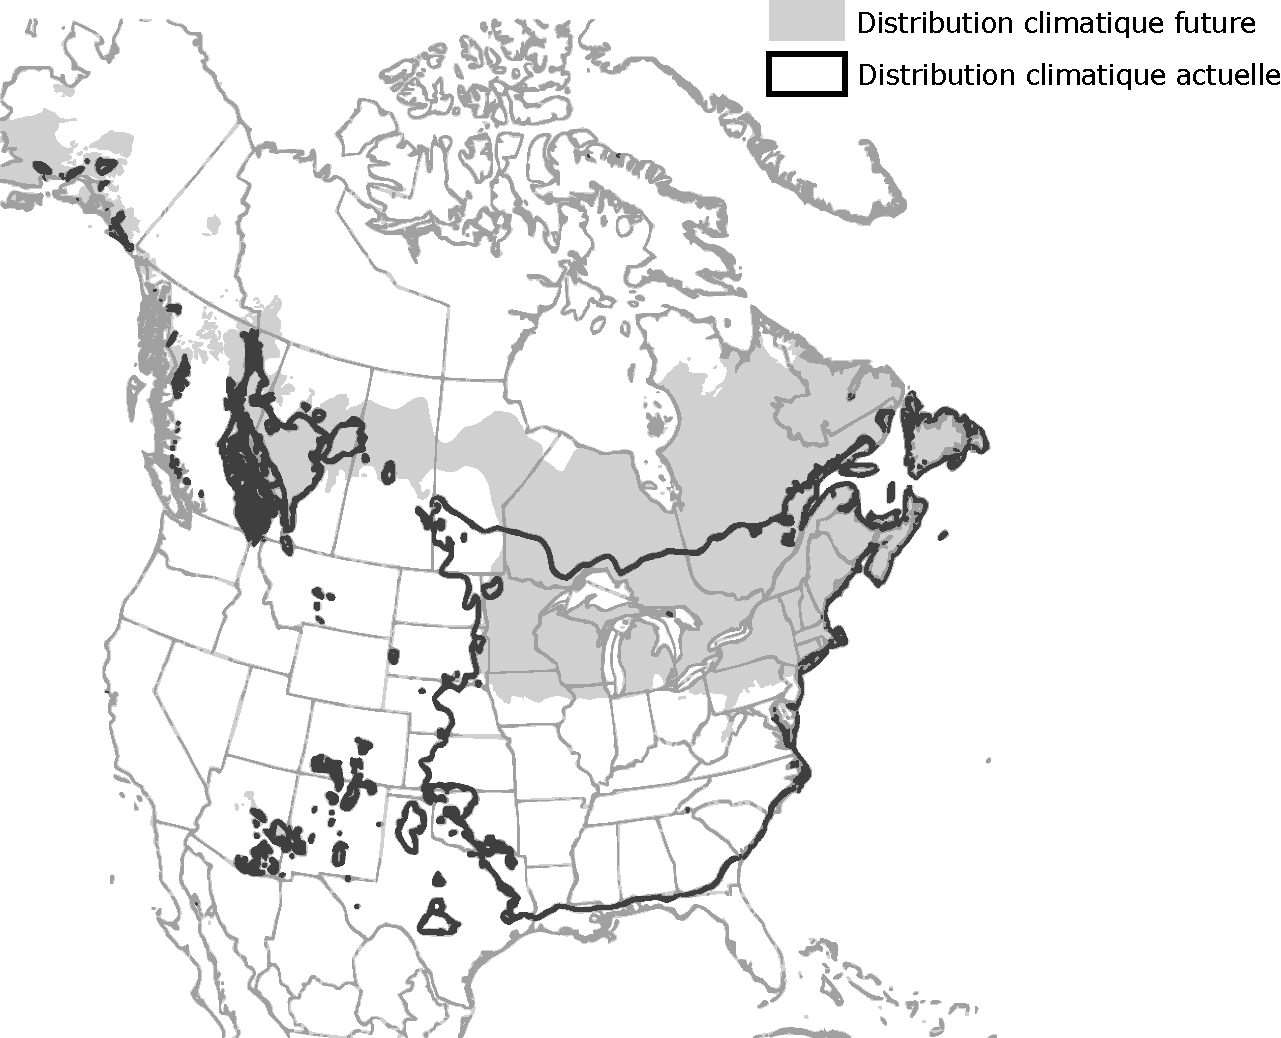
\includegraphics[scale=0.4]{figures/mckenney.pdf}

\par
\stopcols

\smallcitation{McKenney \textit{et al}. 2007 BioScience}

\end{frame}

\begin{frame}{La forêt ne suit pas les changements climatiques}
\protect\hypertarget{la-foruxeat-ne-suit-pas-les-changements-climatiques}{}

\vspace*{-15mm}
\begin{center}
  \begin{tikzpicture}
    \node<1> (img1) {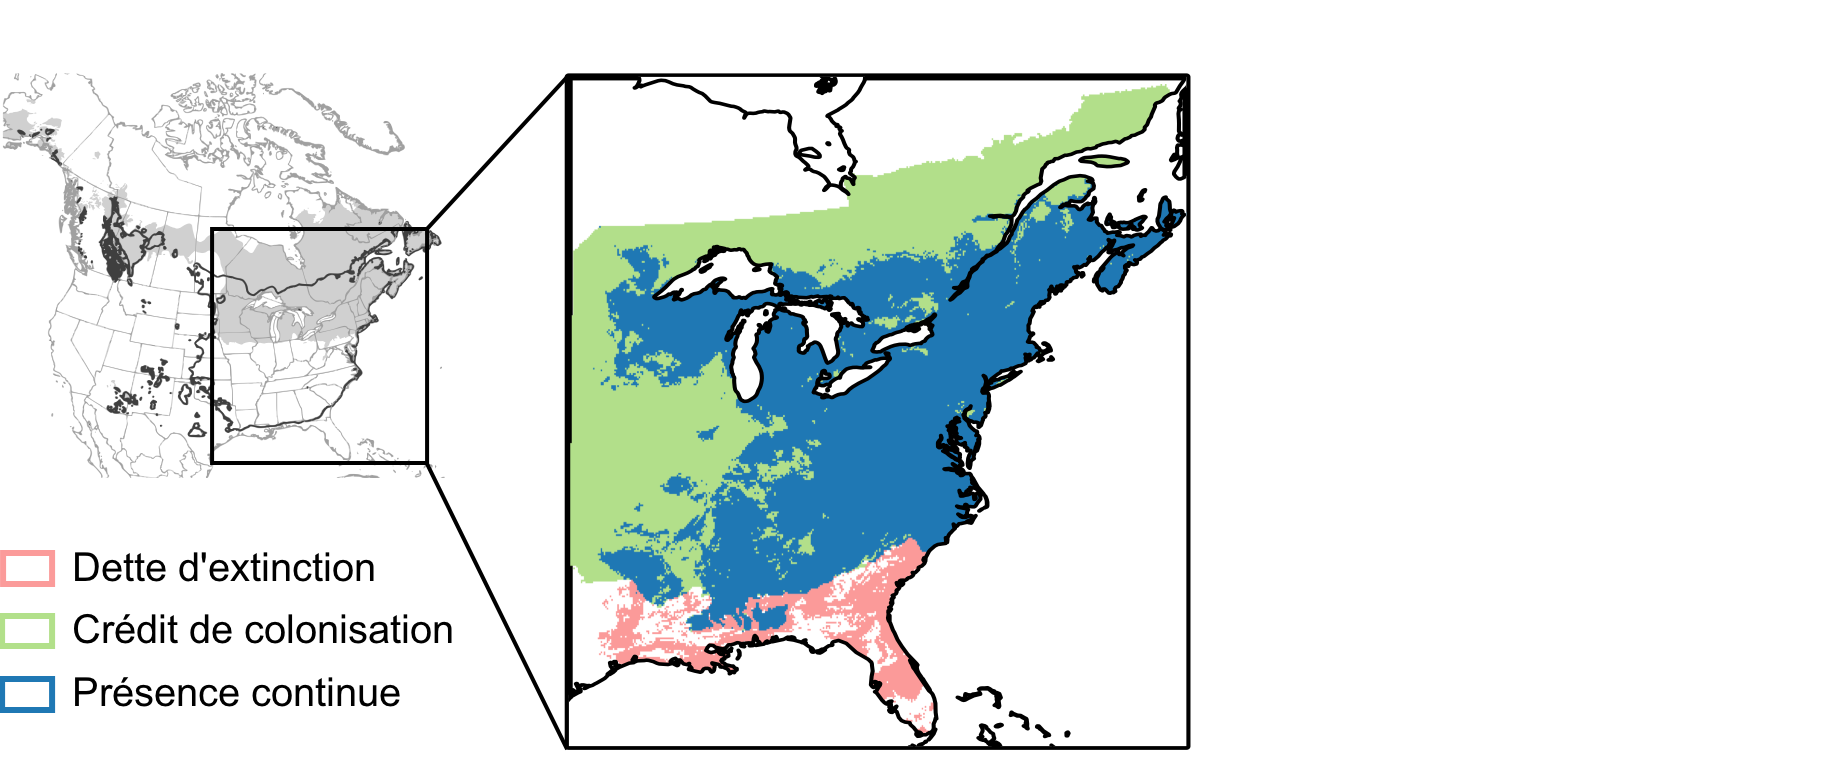
\includegraphics[scale=0.45]{figures/Talluto0.png}};
  \end{tikzpicture}
\end{center}
\smallcitation{Talluto \textit{et al}. 2017 Nat. Ecol. Evol.}

\end{frame}

\begin{frame}{Possibles conséquences}
\protect\hypertarget{possibles-consuxe9quences}{}

\vspace*{-15mm}
\begin{center}
  \begin{tikzpicture}
    \node<1> (img1) {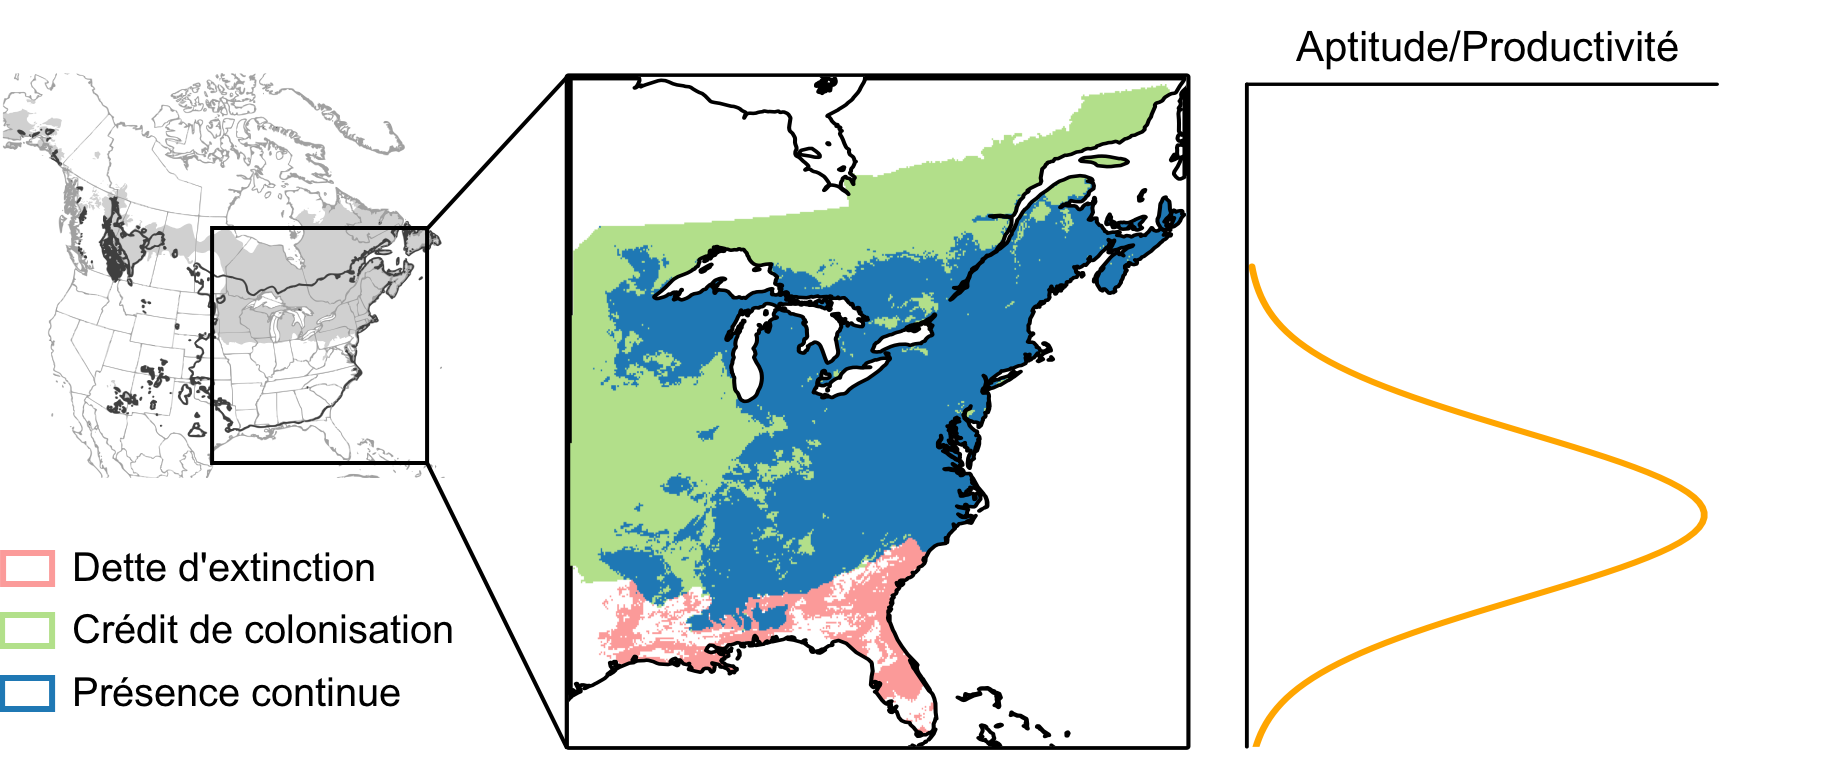
\includegraphics[scale=0.45]{figures/Talluto1.png}};
    \node<2> (img2) {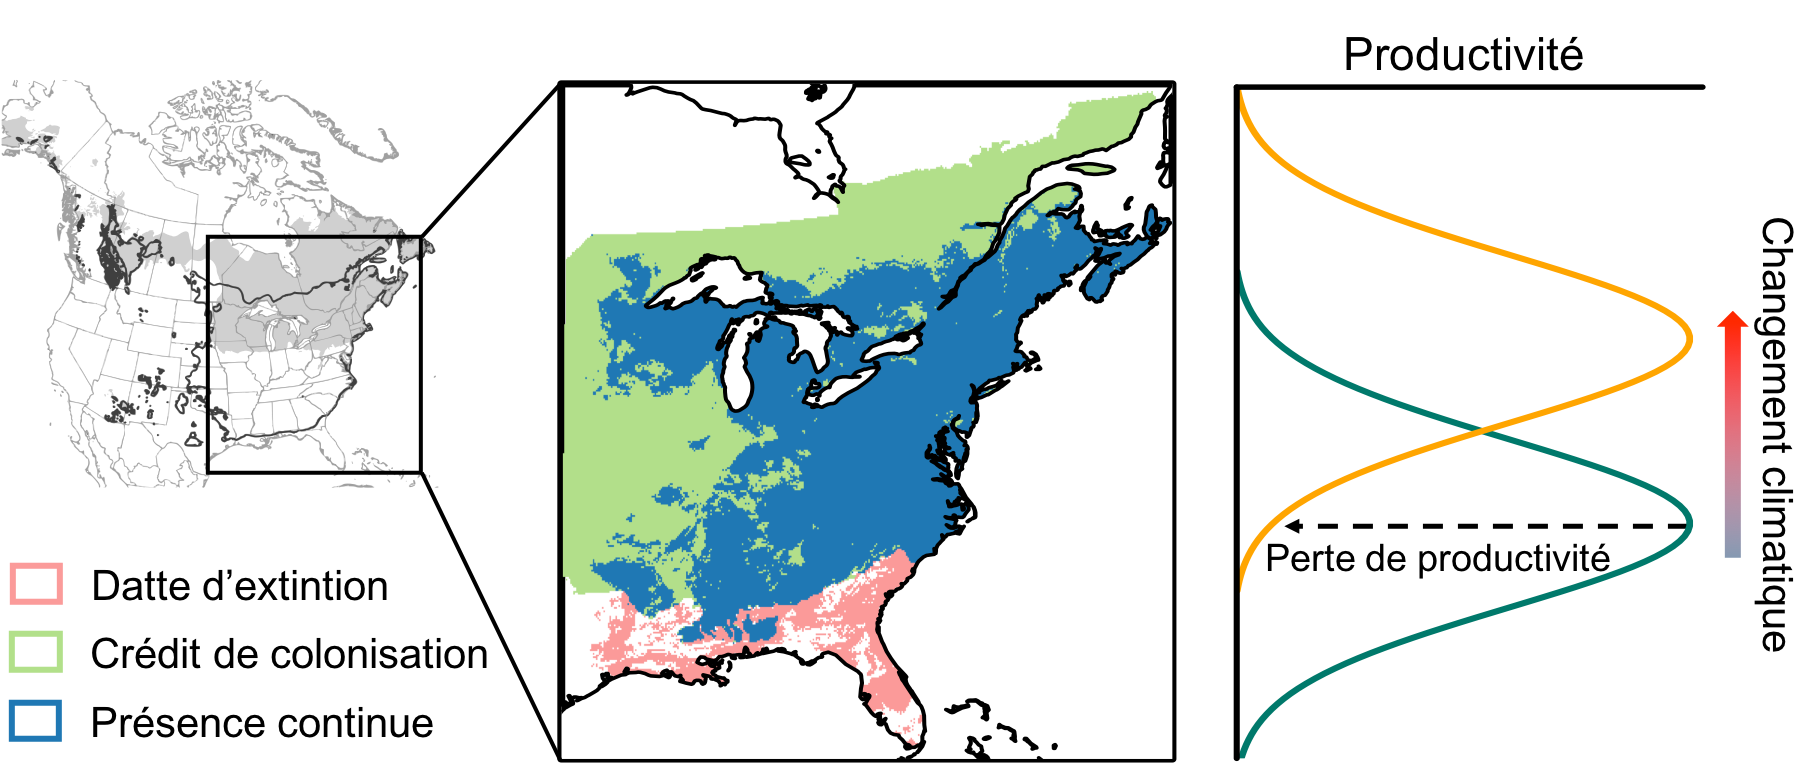
\includegraphics[scale=0.45]{figures/Talluto2.png}};
  \end{tikzpicture}
\end{center}

\end{frame}

\begin{frame}{Cadre théorique - expansion des espèces}
\protect\hypertarget{cadre-thuxe9orique---expansion-des-espuxe8ces}{}

\begin{LARGE}
$$ 2 \times \sqrt{rD} $$
\end{LARGE}

\begin{description}
\tightlist
\item[r]
taux de croissance de la population
\item[D]
coefficient de diffusion
\end{description}

\smallcitation{Skellam 1951 Biometrika}

\end{frame}

\begin{frame}{Cadre théorique - expansion des espèces}
\protect\hypertarget{cadre-thuxe9orique---expansion-des-espuxe8ces-1}{}

\begincols
\column{0.5\textwidth}
\begin{Large}
  \begin{gather*}
    2 \times \sqrt{\alert{r}D} \\
    r = \text{natalité} - \text{mortalité}
  \end{gather*}
\end{Large}

\alert{Démographie} dépendante de l’environnement

\hfill\column{0.5\textwidth}
  \centering

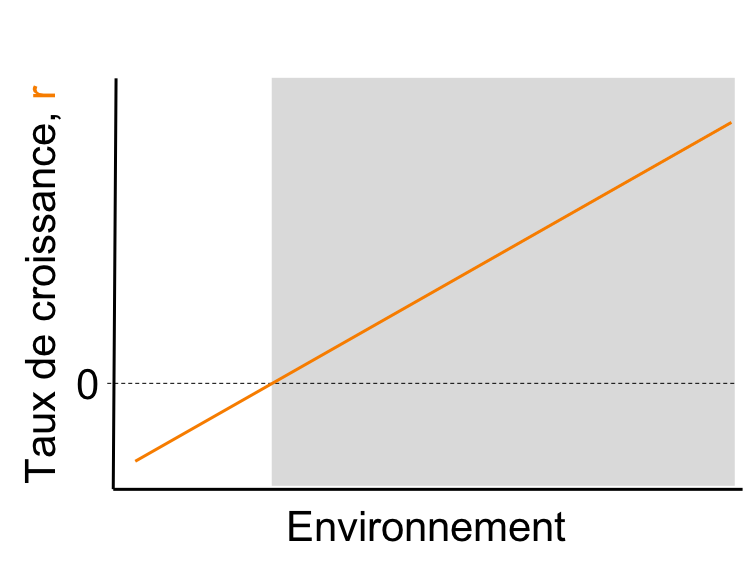
\includegraphics[scale=0.43]{figures/croissance.png}

\par
\stopcols

\end{frame}

\begin{frame}{Cadre théorique - impact des interactions des espèces sur
l’expansion des espèces}
\protect\hypertarget{cadre-thuxe9orique---impact-des-interactions-des-espuxe8ces-sur-lexpansion-des-espuxe8ces}{}

\centering

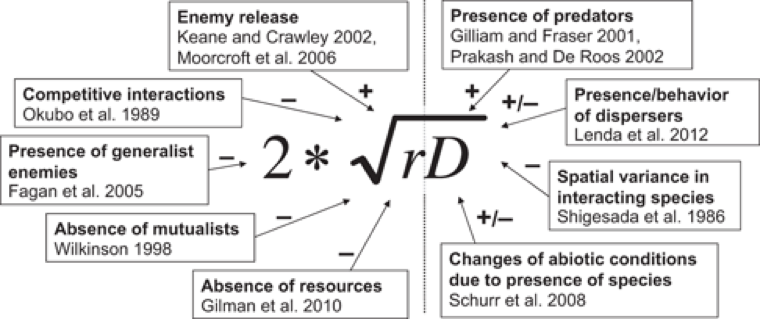
\includegraphics[scale=0.48]{figures/Svenning2014.png}

\par

\end{frame}

\begin{frame}{Cadre théorique - climat et interactions des espèces sur
l’aire de répartition}
\protect\hypertarget{cadre-thuxe9orique---climat-et-interactions-des-espuxe8ces-sur-laire-de-ruxe9partition}{}

\centering

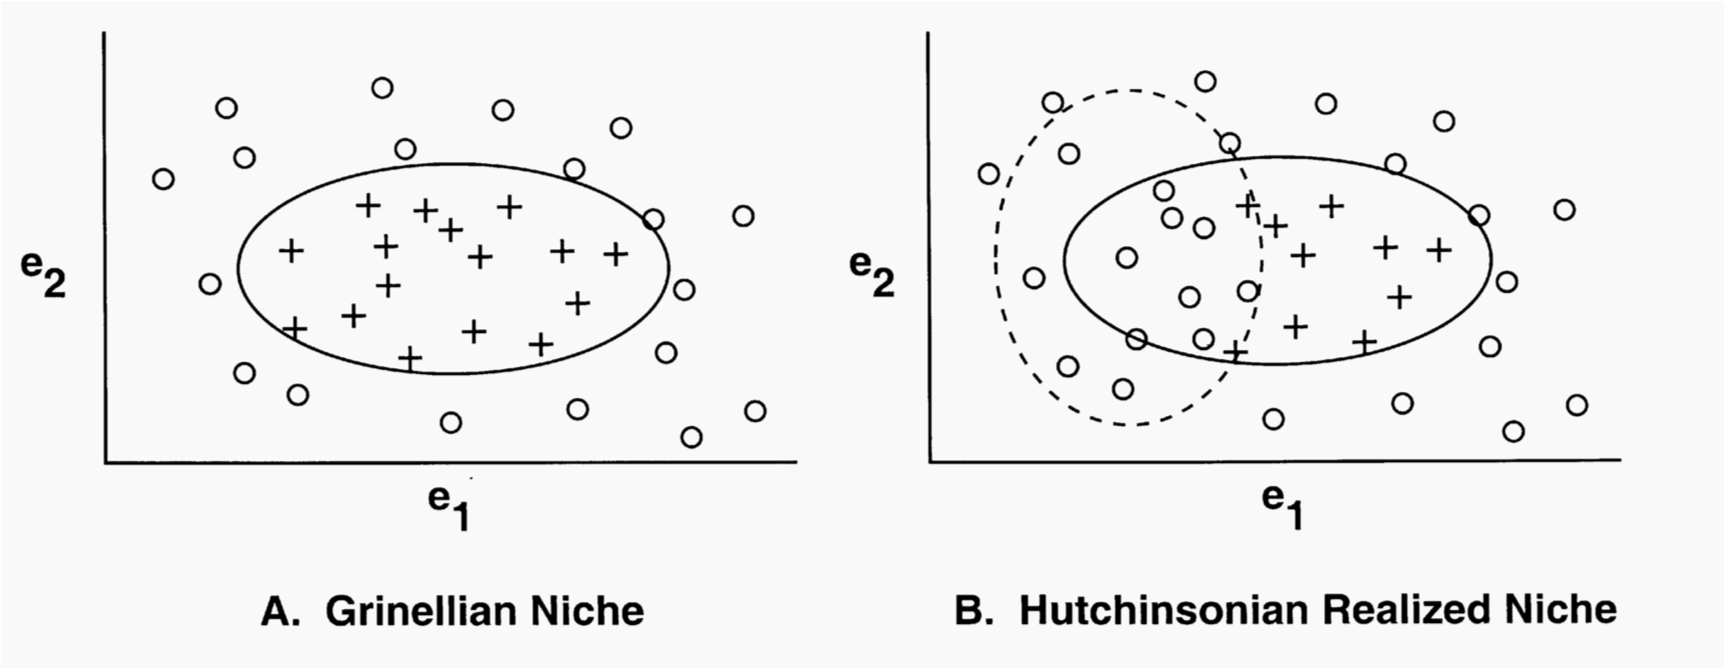
\includegraphics[scale=0.45]{figures/Pulliam2000.png}

\par

\smallcitation{Pulliam et al. 2000 Ecol. Lett.}

\end{frame}

\begin{frame}{Cadre théorique - Intégration de l’aménagement forestier}
\protect\hypertarget{cadre-thuxe9orique---intuxe9gration-de-lamuxe9nagement-forestier}{}

\begincols
\column{0.18\textwidth}
  \vspace*{4.5mm}
  \hspace{10mm}
  \centering

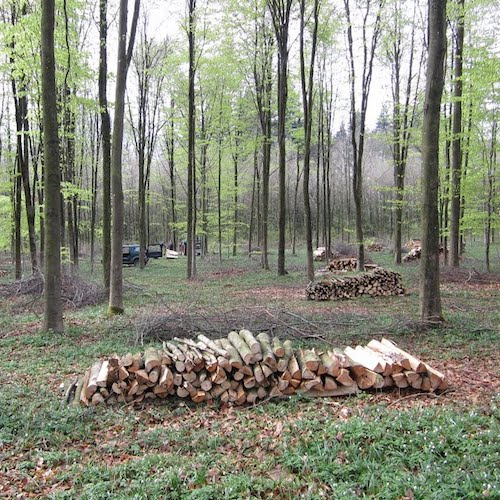
\includegraphics[scale=0.15]{figures/eclarcie.jpg}

\par

\hfill\column{0.4\textwidth}
  \centering
    \begin{center}
  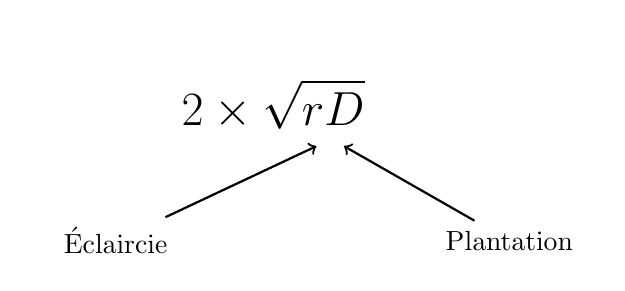
\begin{tikzpicture}[thick,every text node part/.style={align=center}]

    % --------------------------------------------------------- %
    % ------------- principal node (Formula)
    % --------------------------------------------------------- %
    \node[text width=6cm,minimum height=1cm,minimum width=3cm] (formule) at (10,10) {\LARGE{$$2 \times \sqrt{rD}$$}};

    % --------------------------------------------------------- %
    % ------------ Effect of forst management
    % --------------------------------------------------------- %
    \node[text width=2cm] (ecl) at (8,8) {Éclaircie};
    \draw[->]	(ecl) to node [midway] (formule) {} (10.55,9.2);

    \node[text width=2cm] (plant) at (13,8) {Plantation};
    \draw [->] (plant) to node [midway] (formule) {} (10.9,9.2);

  \end{tikzpicture}
\end{center}
\par

\hfill\column{0.4\textwidth}
    \centering

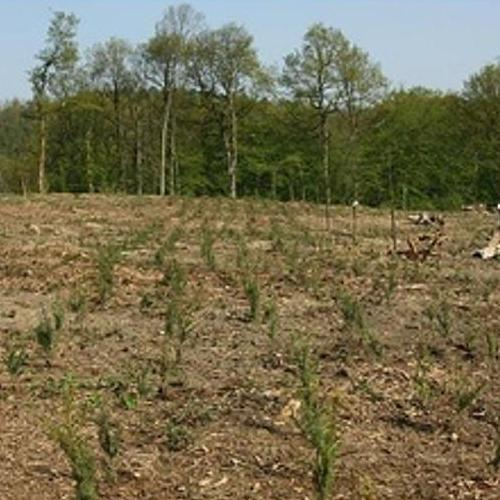
\includegraphics[scale=0.15]{figures/plantation.jpg}

\par
\stopcols

\end{frame}

\begin{frame}{Objectifs}
\protect\hypertarget{objectifs}{}

\vspace*{-15mm}
\begin{center}
  \hspace*{-12mm}
  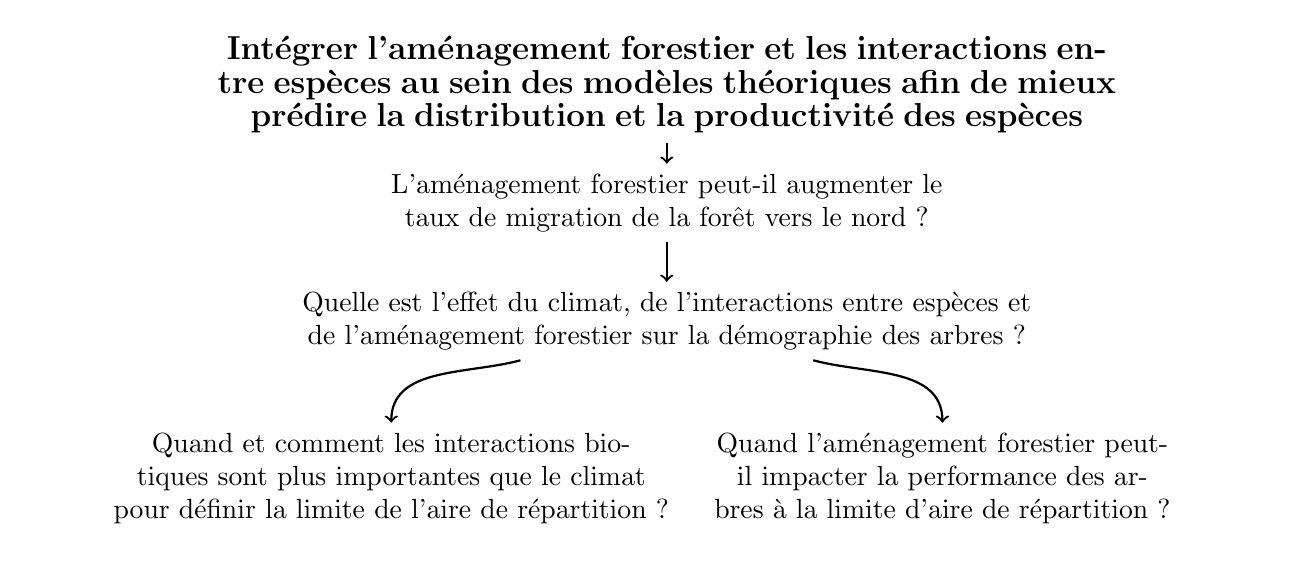
\begin{tikzpicture}[thick,every text node part/.style={align=center}]

    % --------------------------------------------------------- %
    % ------------- principal node (question)
    % --------------------------------------------------------- %
    \node[text width=15cm] (question) at (10,10.25) {\textbf{\large Intégrer l'aménagement forestier et les interactions entre espèces au sein des modèles théoriques afin de mieux prédire la distribution et la productivité des espèces}};

    % --------------------------------------------------------- %
    % ------------ Objectives
    % --------------------------------------------------------- %
    % --- Obj0 node
    \node[text width=12cm,visible on=<2->] (obj0) at (10,8.75) {L'aménagement forestier peut-il augmenter le taux de migration de la forêt vers le nord ?};
    \draw [->,visible on=<2->] (question) edge [out=270, in=90] (obj0);
    % --- Obj1 node
    \node[text width=12cm,visible on=<3->] (obj1) at (10,7.25) {Quelle est l'effet du climat, de l'interactions entre espèces et de l'aménagement forestier sur la démographie des arbres ?};
    \draw [->,visible on=<3->] (obj0) edge [out=270, in=90] (obj1);
    % --- Obj2 node
    \node[text width=9cm,visible on=<4->] (obj2) at (6.5,5.25) {Quand et comment les interactions biotiques sont plus importantes que le climat pour définir la limite de l'aire de répartition ?};
    \draw [->,visible on=<4->] (obj1) edge [out=195, in=90] (obj2);
    % --- Obj2 node
    \node[text width=8cm,visible on=<5->] (obj3) at (13.5,5.25) {Quand l'aménagement forestier peut-il impacter la performance des arbres à la limite d'aire de répartition ?};
    \draw [->,visible on=<5->] (obj1) edge [out=345, in=90] (obj3);
    % --- Obj3 node

  \end{tikzpicture}
\end{center}


\end{frame}

\hypertarget{chapitre-i-impact-de-lamuxe9nagement-forestier-sur-le-taux-de-migration-des-foruxeats-de-lamuxe9rique-du-nord}{%
\section{\texorpdfstring{Chapitre I: \newline Impact de l’aménagement
forestier sur le taux de migration des forêts de l’Amérique du
Nord}{Chapitre I: Impact de l’aménagement forestier sur le taux de migration des forêts de l’Amérique du Nord}}\label{chapitre-i-impact-de-lamuxe9nagement-forestier-sur-le-taux-de-migration-des-foruxeats-de-lamuxe9rique-du-nord}}

\begin{frame}{Contexte - objectif}
\protect\hypertarget{contexte---objectif}{}

\begin{center}
  \begin{tikzpicture}
    \node<1> (img1) {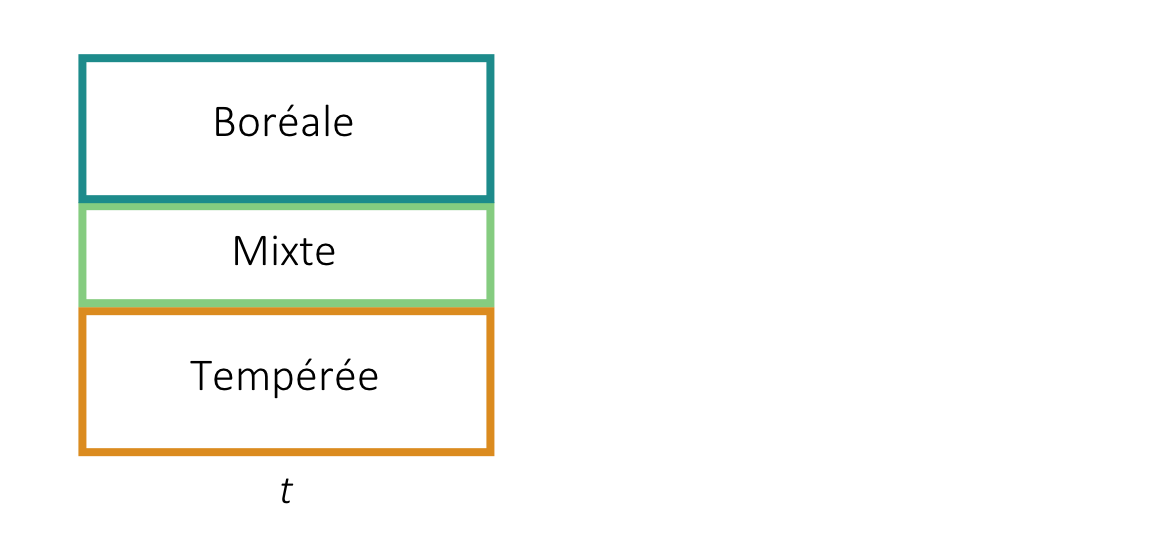
\includegraphics[scale=0.65]{figures/migration0.png}};
    \node<2> (img2) {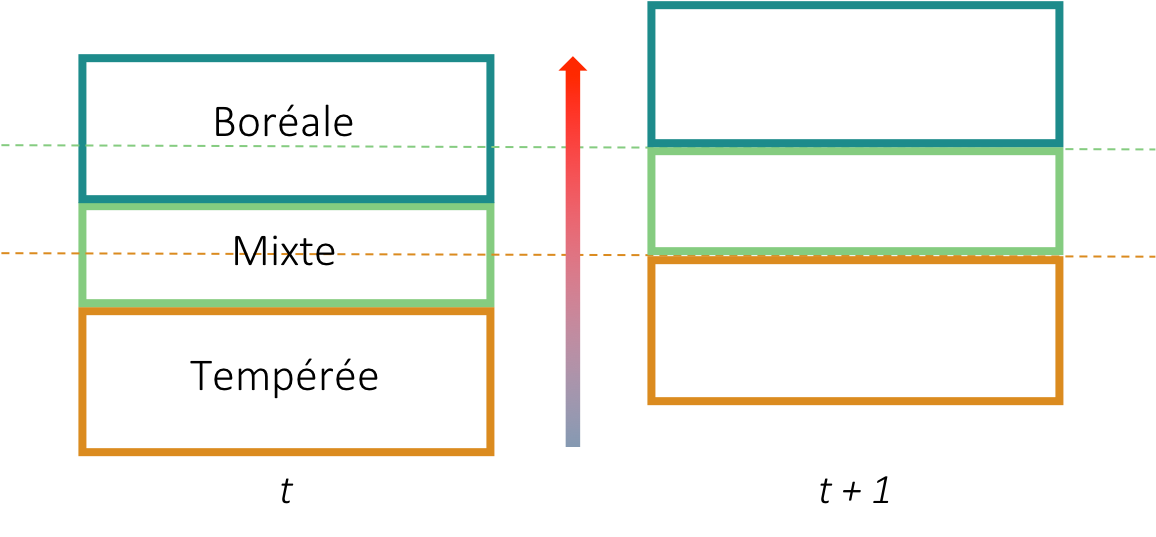
\includegraphics[scale=0.65]{figures/migration.png}};
    \node<3> (img3) {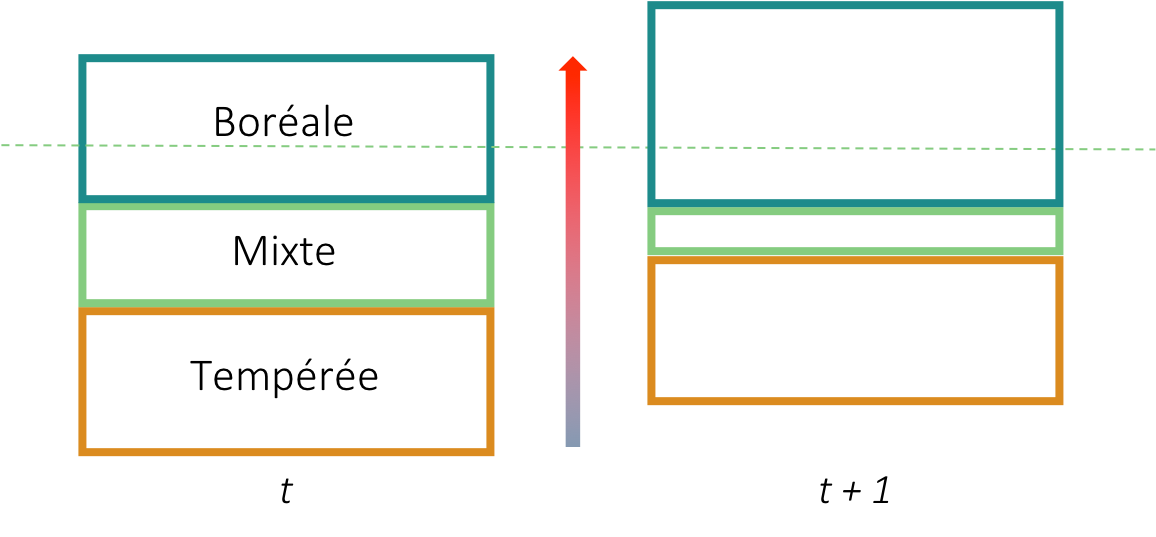
\includegraphics[scale=0.65]{figures/migration1.png}};
    \node<4> (img4) {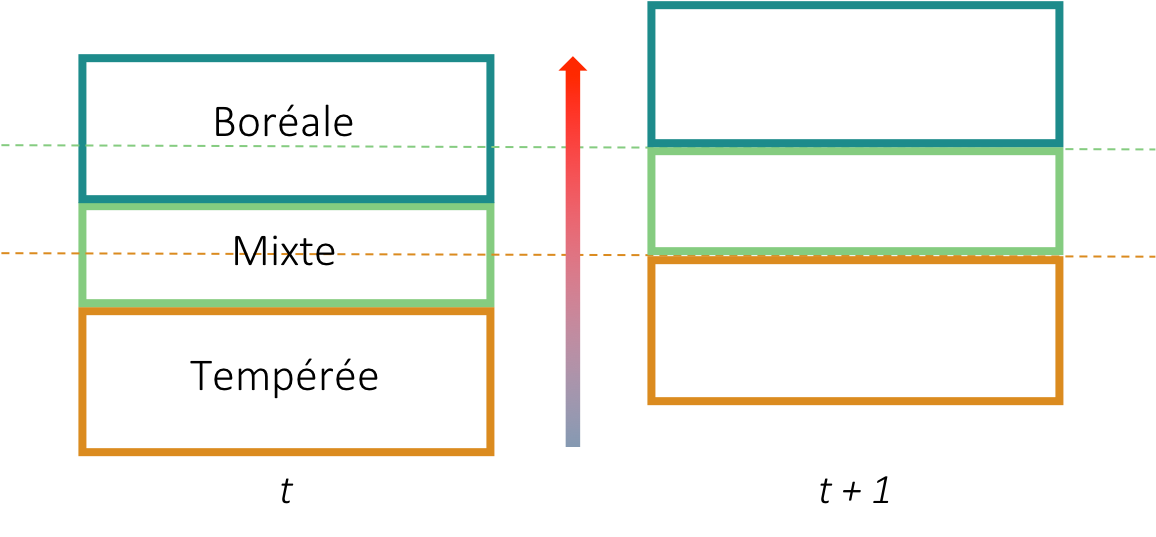
\includegraphics[scale=0.65]{figures/migration.png}};
  \end{tikzpicture}
\end{center}

\end{frame}

\begin{frame}{Modèle de transition d’état}
\protect\hypertarget{moduxe8le-de-transition-duxe9tat}{}

\begincols
\column{0.58\textwidth}
  	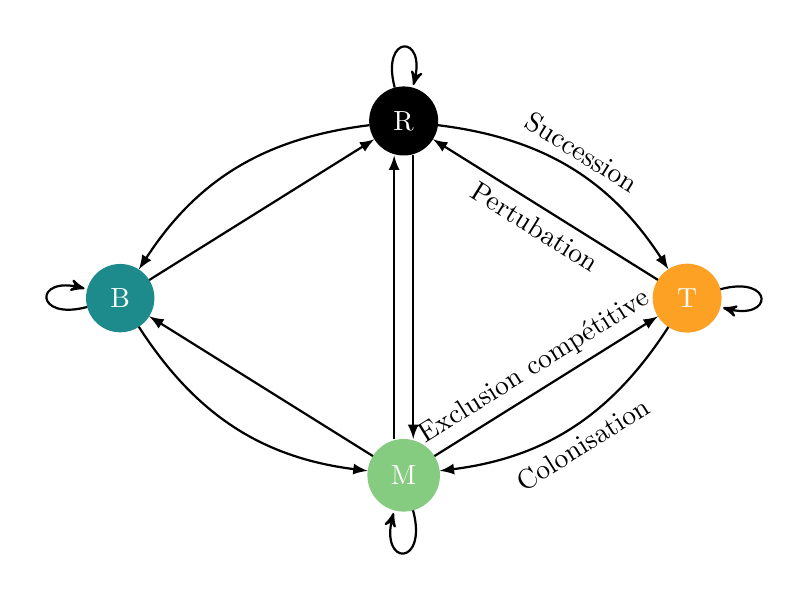
\begin{tikzpicture}[->,>=stealth',auto,scale=0.45]
		\node [circle,StateM] (M) at (0,0) {\textcolor{white}{M}};
		\node [circle,StateB] (B) at (-8,5) {\textcolor{white}{B}};
		\node [circle,StateT] (T) at (8,5) {\textcolor{white}{T}};
		\node [circle,StateR] (R) at (0,10) {\textcolor{white}{R}};

		\path	(M) edge [thick,loop below,-latex]  node {} (M);
		\path	(T) edge [thick,loop right,-latex]  node {} (T);
		\path	(B) edge [thick,loop left,-latex]  node {} (B);
		\path	(R) edge [thick,loop above,-latex]  node {} (R);

		\draw[thick,-latex] (M) to node[above,sloped] {} (B);
		\draw[thick,-latex] (B) to[bend right=25] node[below,sloped] {} (M);

		\draw[thick,-latex] (T) to[bend left=25] node[below,sloped] {Colonisation} (M);
		\draw[thick,-latex] (M) to node[above,sloped] {Exclusion compétitive} (T);

		\draw[thick,-latex] (R) to[bend left=25] node[above,sloped] {Succession} (T);
		\draw[thick,-latex] (T) to node[below,sloped] {Pertubation} (R);

		\draw[thick,-latex] (R) to[bend right=25] node[above,sloped] {} (B);
		\draw[thick,-latex] (B) to node[below,sloped] {} (R);

		\draw[thick,-latex,transform canvas={xshift=0.8ex}] (R) to node[above,sloped] {} (M);
		\draw[thick,-latex,transform canvas={xshift=-0.8ex}] (M) to node[above,sloped] {} (R);
	\end{tikzpicture}

\hfill\column{0.25\textwidth}
\vspace{-5mm}

\begin{itemize}
    \item
      \textbf{\textcolor{cB}{B}}oréale
    \item
      \textbf{\textcolor{cM}{M}}ixte
    \item
      \textbf{\textcolor{cT}{T}}empérée
    \item
    \textbf{\textcolor{cR}{R}}égeneration
  \end{itemize}

\stopcols

\smallcitation{Vissault et al. submitted}

\end{frame}

\begin{frame}{Pratiques d’aménagement considérées dans le modèle}
\protect\hypertarget{pratiques-damuxe9nagement-considuxe9ruxe9es-dans-le-moduxe8le}{}

\begincols
\column{0.28\textwidth}

\textbf{Aménagement forestier}

\begin{enumerate}

    \tightlist
    \item
      Plantation
    \item
      Coupe
    \item
      Coupe sélective
    \item
      Enrichissement
  \end{enumerate}

\hfill\column{0.55\textwidth}
    \centering

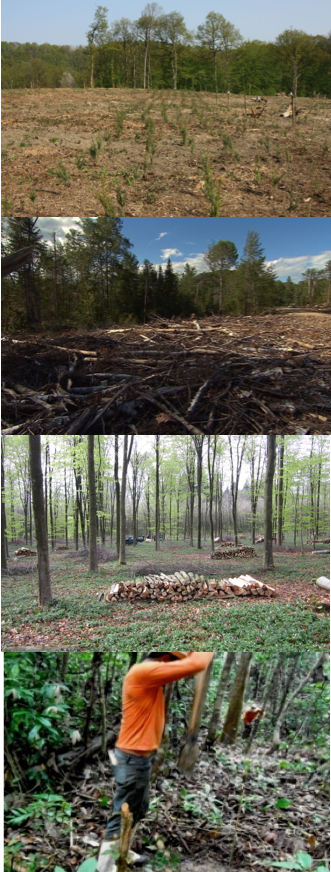
\includegraphics[scale=0.50]{figures/managPrac}

\par
\stopcols

\end{frame}

\begin{frame}{Intégration avec l’aménagement forestier}
\protect\hypertarget{intuxe9gration-avec-lamuxe9nagement-forestier}{}

\centering

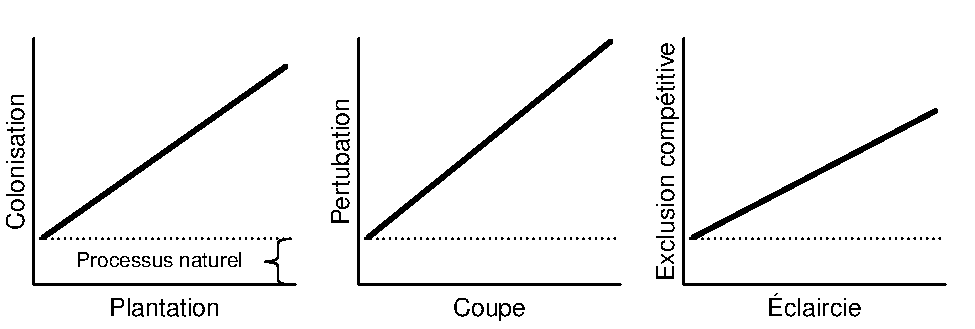
\includegraphics[scale=0.65]{figures/managMechanism.pdf}

\par

\end{frame}

\begin{frame}{Intégration avec l’aménagement forestier}
\protect\hypertarget{intuxe9gration-avec-lamuxe9nagement-forestier-1}{}

\centering
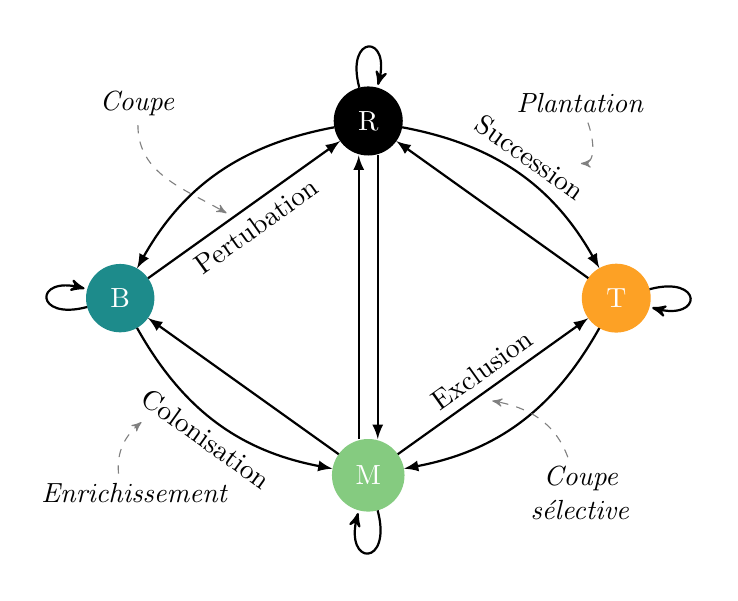
\begin{tikzpicture}[->,>=stealth',auto,scale=0.45]
  \node [circle,StateM] (M) at (0,0) {\textcolor{white}{M}};
  \node [circle,StateB] (B) at (-7,5) {\textcolor{white}{B}};
  \node [circle,StateT] (T) at (7,5) {\textcolor{white}{T}};
  \node [circle,StateR] (R) at (0,10) {\textcolor{white}{R}};

  \path	(M) edge [thick,loop below,-latex]  node {} (M);
  \path	(T) edge [thick,loop right,-latex]  node {} (T);
  \path	(B) edge [thick,loop left,-latex]  node {} (B);
  \path	(R) edge [thick,loop above,-latex]  node {} (R);

  % management nodes
  \node [text width=2cm,align=center] (plant) at (6,10.5) {\textit{Plantation}};
  \node [text width=2cm,align=center] (harv) at (-6.5,10.5) {\textit{Coupe}};
  \node [text width=2cm,align=center] (thin) at (6,-0.5) {\textit{Coupe sélective}};
  \node [text width=2cm,align=center] (enrich) at (-7,-0.5) {\textit{Enrichissement}};

  \draw[thick,-latex] (M) to node[above,sloped] {} (B);
  \draw[thick,-latex] (B) to[bend right=25] node[below,sloped] {Colonisation} (M);

  \draw[thick,-latex] (T) to[bend left=25] node[below,sloped] {} (M);
  \draw[thick,-latex] (M) to node[above,sloped] {Exclusion} (T);

  \draw[thick,-latex] (R) to[bend left=25] node[above,sloped] {Succession} (T);
  \draw[thick,-latex] (T) to node[below,sloped] {} (R);

  \draw[thick,-latex] (R) to[bend right=25] node[above,sloped] {} (B);
  \draw[thick,-latex] (B) to node[below,sloped] {Pertubation} (R);

  \draw[thick,-latex,transform canvas={xshift=0.8ex}] (R) to node[above,sloped] {} (M);
  \draw[thick,-latex,transform canvas={xshift=-0.8ex}] (M) to node[above,sloped] {} (R);

  % add management arrows
  \draw [gray,dashed,->] (plant) edge [out=290, in=0] (6,8.8);
  \draw [gray,dashed,->] (harv) edge [out=270, in=150] (-4,7.4);
  \draw [gray,dashed,->] (enrich) edge [out=95, in=220] (-6.4,1.5);
  \draw [gray,dashed,->] (thin) edge [out=110, in=350] (3.5,2.1);

\end{tikzpicture}
\par

\end{frame}

\begin{frame}{Analyse analytique}
\protect\hypertarget{analyse-analytique}{}

\begincols
\column{0.4\textwidth}

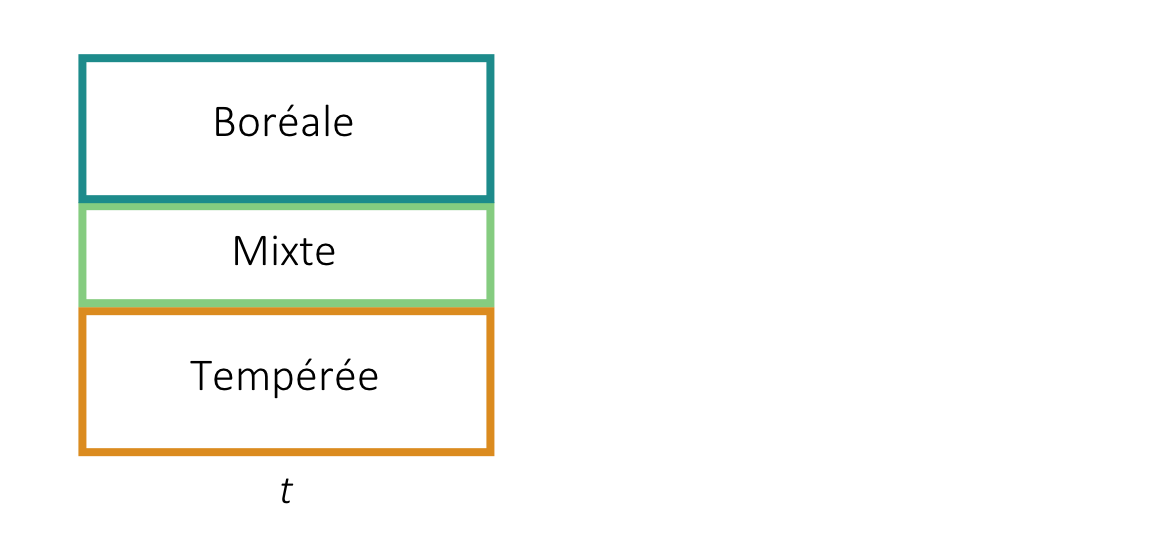
\includegraphics[scale=0.50]{figures/migration0.png}
\hfill\column{0.5\textwidth}
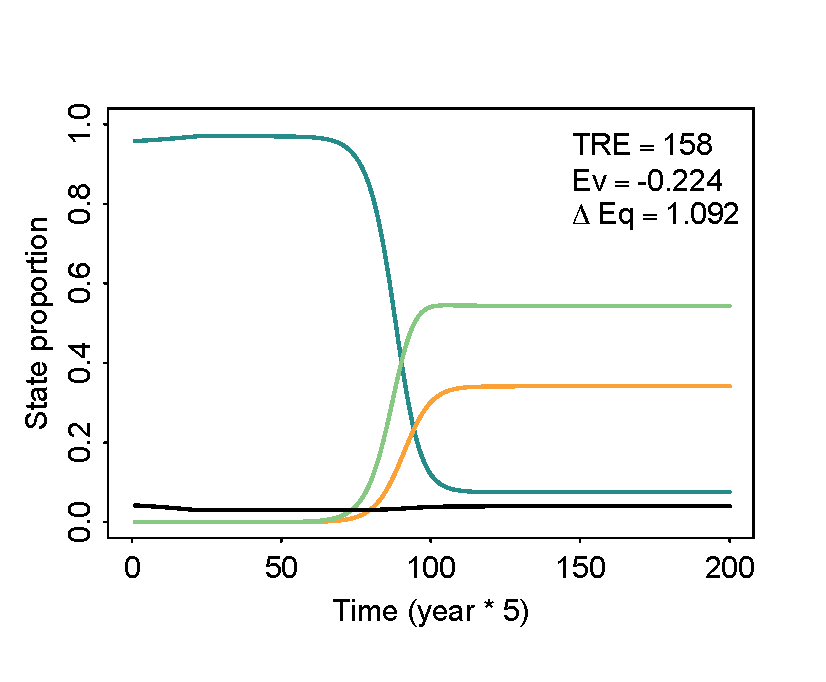
\includegraphics[scale=0.55]{figures/analyticalAnalysis} \stopcols

\end{frame}

\begin{frame}{Analyse par simulations}
\protect\hypertarget{analyse-par-simulations}{}

\begincols
\column{0.4\textwidth}

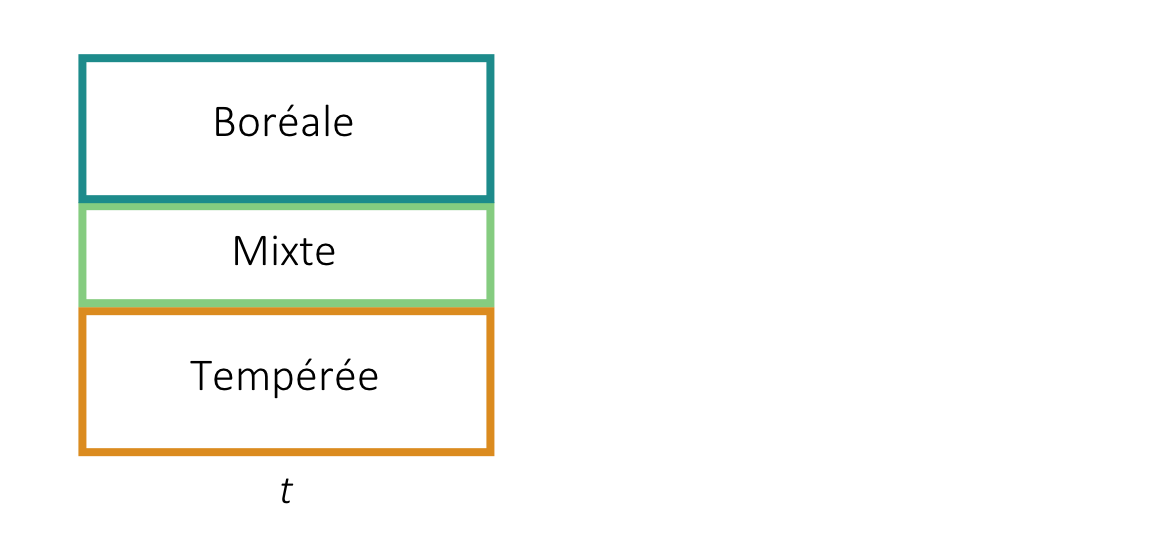
\includegraphics[scale=0.50]{figures/migration0.png}
\hfill\column{0.5\textwidth}
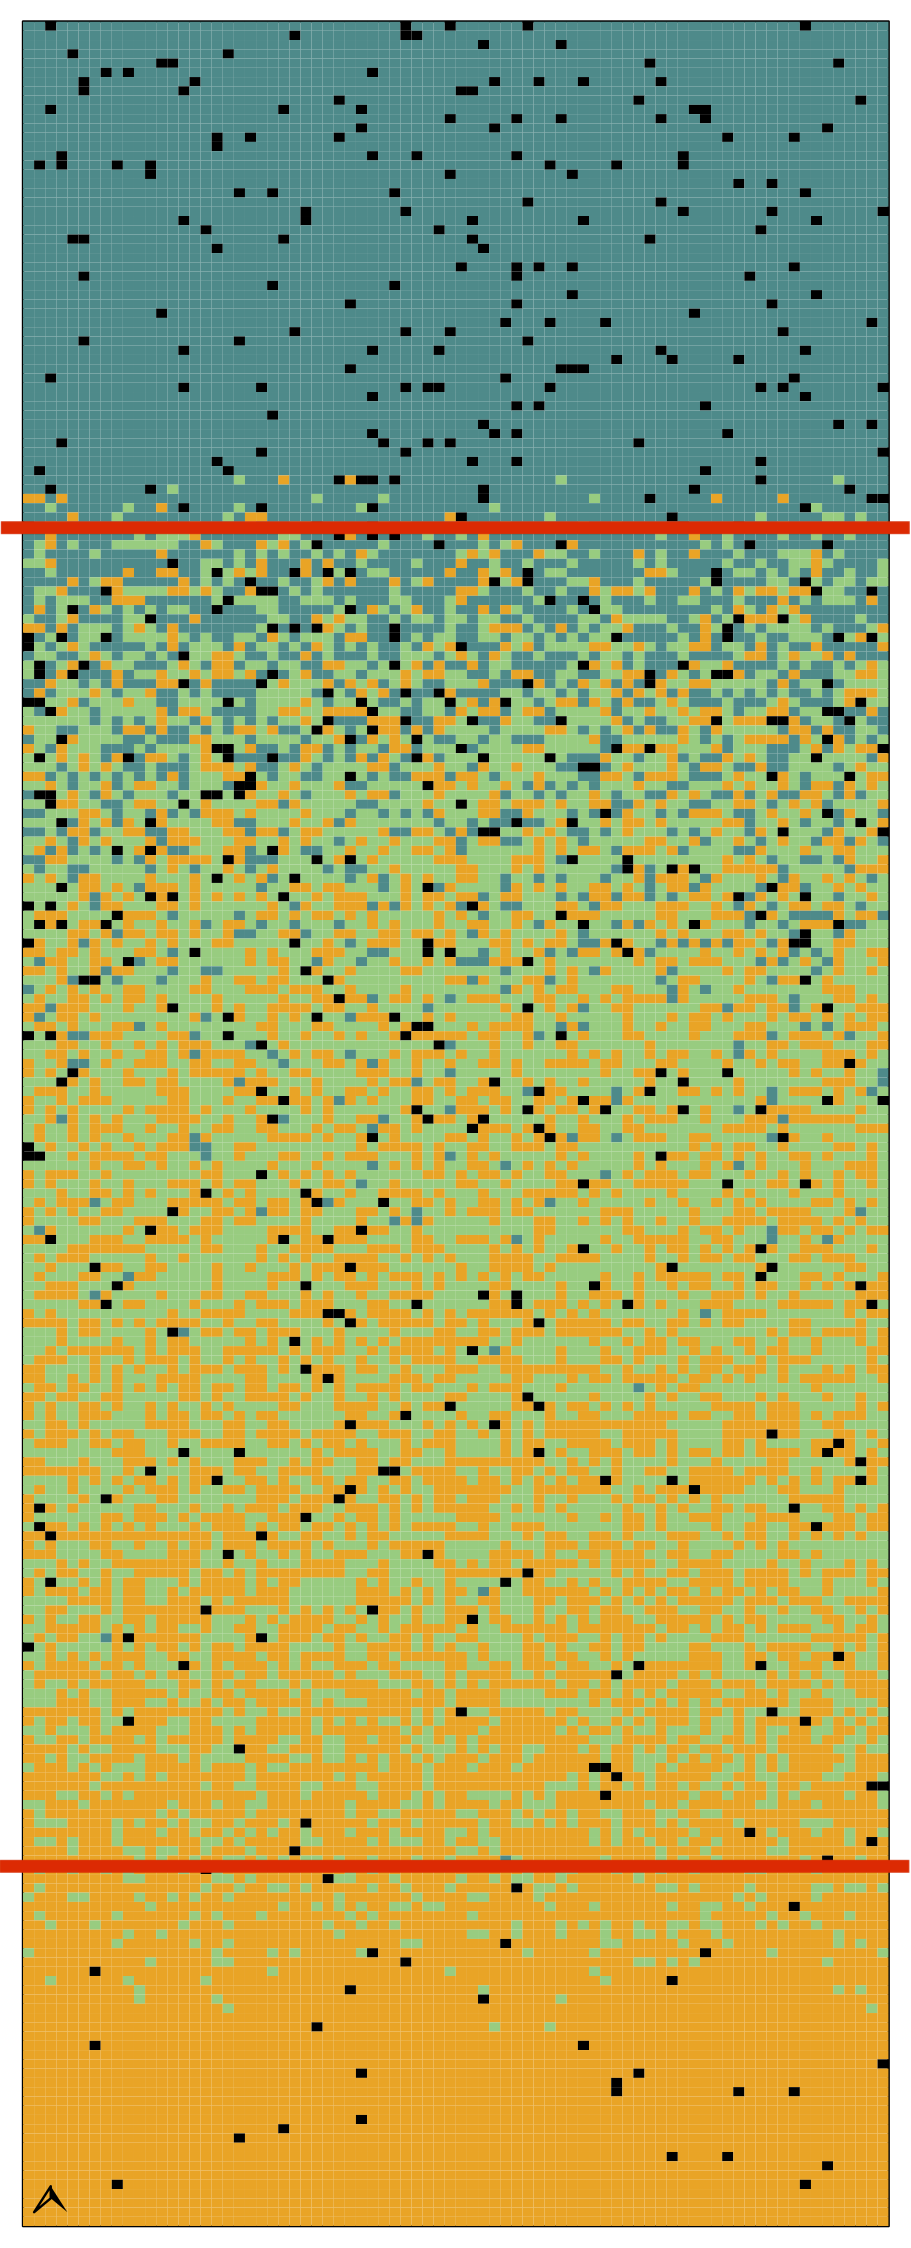
\includegraphics[scale=0.32]{figures/initLand}

\par
\stopcols

\end{frame}

\begin{frame}{Résultats préliminaires - analytique}
\protect\hypertarget{ruxe9sultats-pruxe9liminaires---analytique}{}

Effet de l’aménagement forestier sur le \textbf{temps pour arriver à
l’equilibre}

\centering

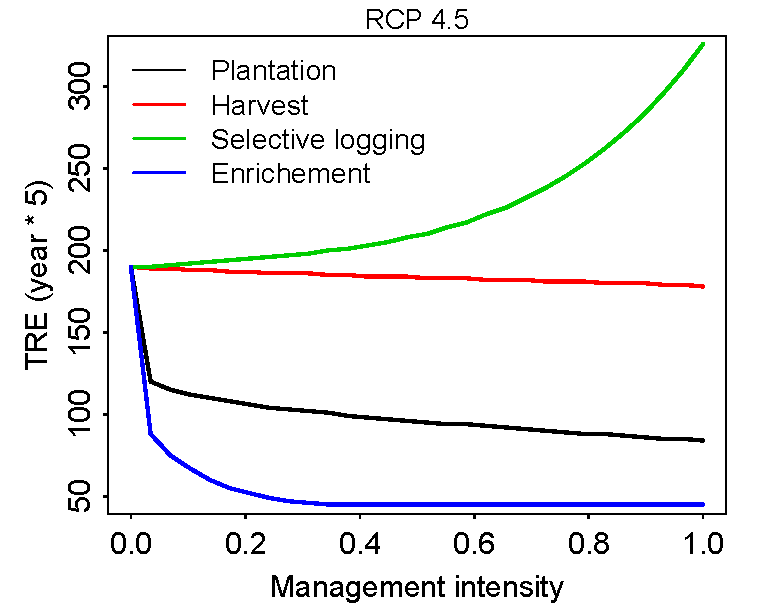
\includegraphics[scale=0.55]{figures/resultTRE.pdf}

\par

\end{frame}

\begin{frame}{Résultats préliminaires - simulations}
\protect\hypertarget{ruxe9sultats-pruxe9liminaires---simulations}{}

\vspace*{-6mm}
\centering

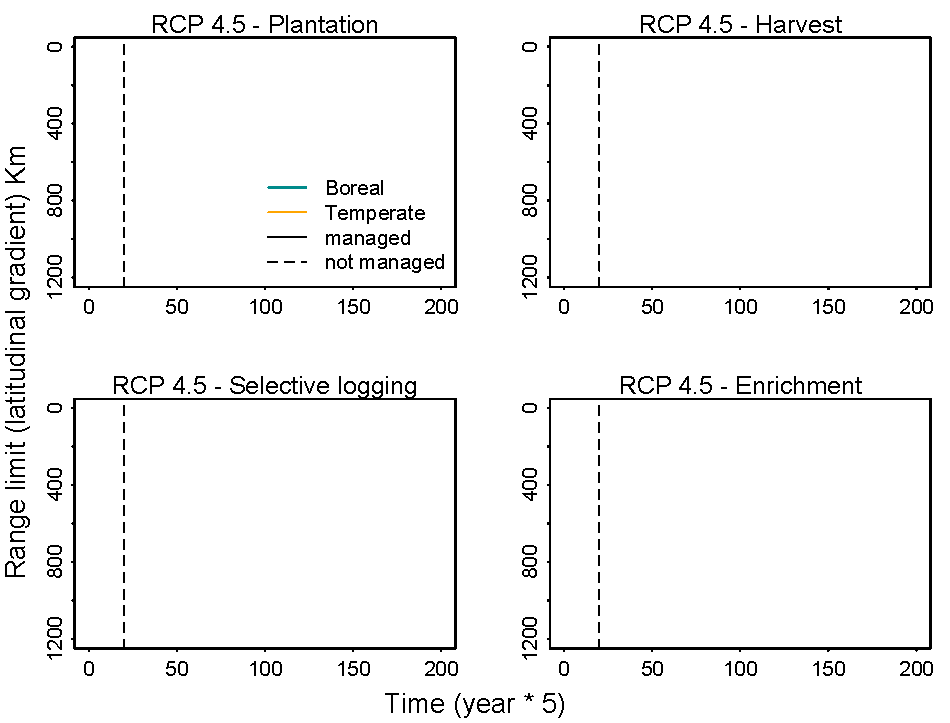
\includegraphics[scale=0.65]{figures/resultSim0.pdf}

\par

\end{frame}

\begin{frame}{Résultats préliminaires - simulations}
\protect\hypertarget{ruxe9sultats-pruxe9liminaires---simulations-1}{}

\vspace*{-6mm}
\centering

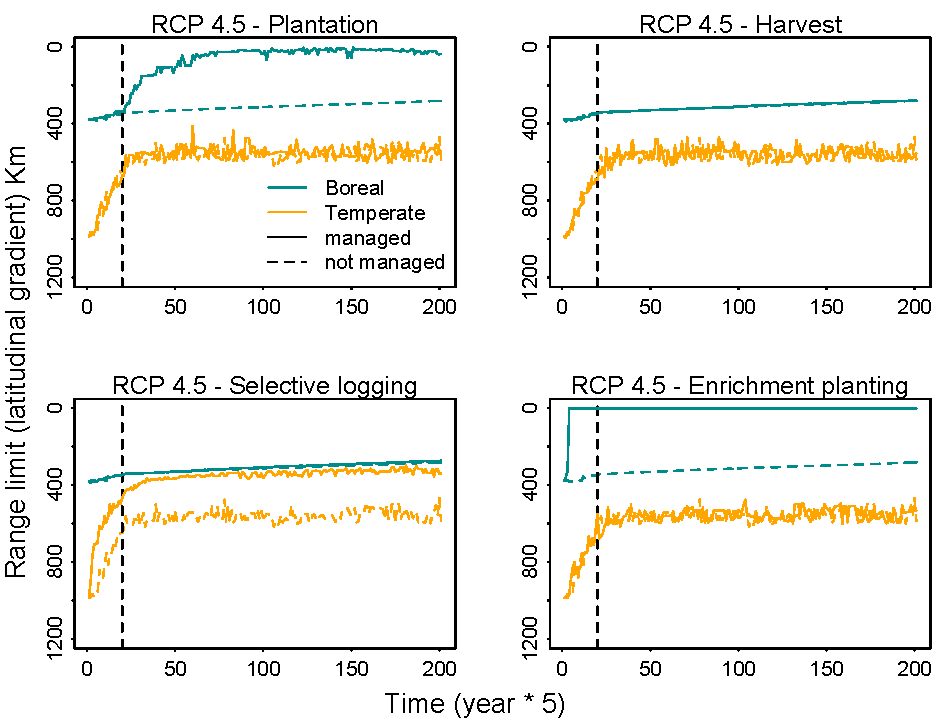
\includegraphics[scale=0.65]{figures/resultSim.pdf}

\par

\end{frame}

\hypertarget{chapitre-ii-le-moduxe8le-de-projection-intuxe9grale-ipm-leffet-du-climat-et-de-linteraction-entre-espuxe8ces-sur-la-duxe9mographie-des-arbres}{%
\section{\texorpdfstring{Chapitre II: \newline Le modèle de projection
intégrale (IPM) \newline \large L’effet du climat et de l’interaction
entre espèces sur la démographie des
arbres}{Chapitre II: Le modèle de projection intégrale (IPM) L’effet du climat et de l’interaction entre espèces sur la démographie des arbres}}\label{chapitre-ii-le-moduxe8le-de-projection-intuxe9grale-ipm-leffet-du-climat-et-de-linteraction-entre-espuxe8ces-sur-la-duxe9mographie-des-arbres}}

\begin{frame}{Dynamiques forestières à différentes échelles spatiales}
\protect\hypertarget{dynamiques-forestiuxe8res-uxe0-diffuxe9rentes-uxe9chelles-spatiales}{}

\begin{columns}[T]
  \column{6.5cm}
    1. Locale

    \centering
      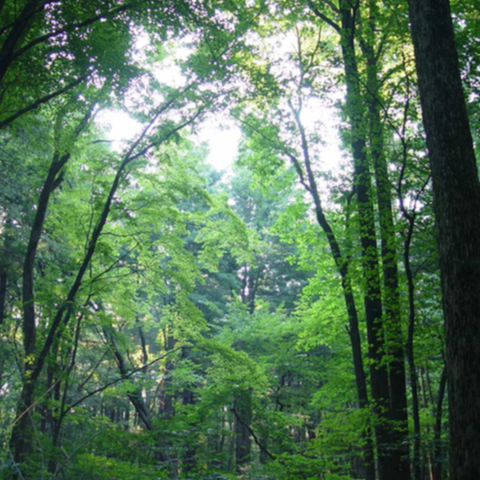
\includegraphics[scale=0.338]{figures/gap}\par
  \column{6.5cm}
    2. Régionale

    \centering
      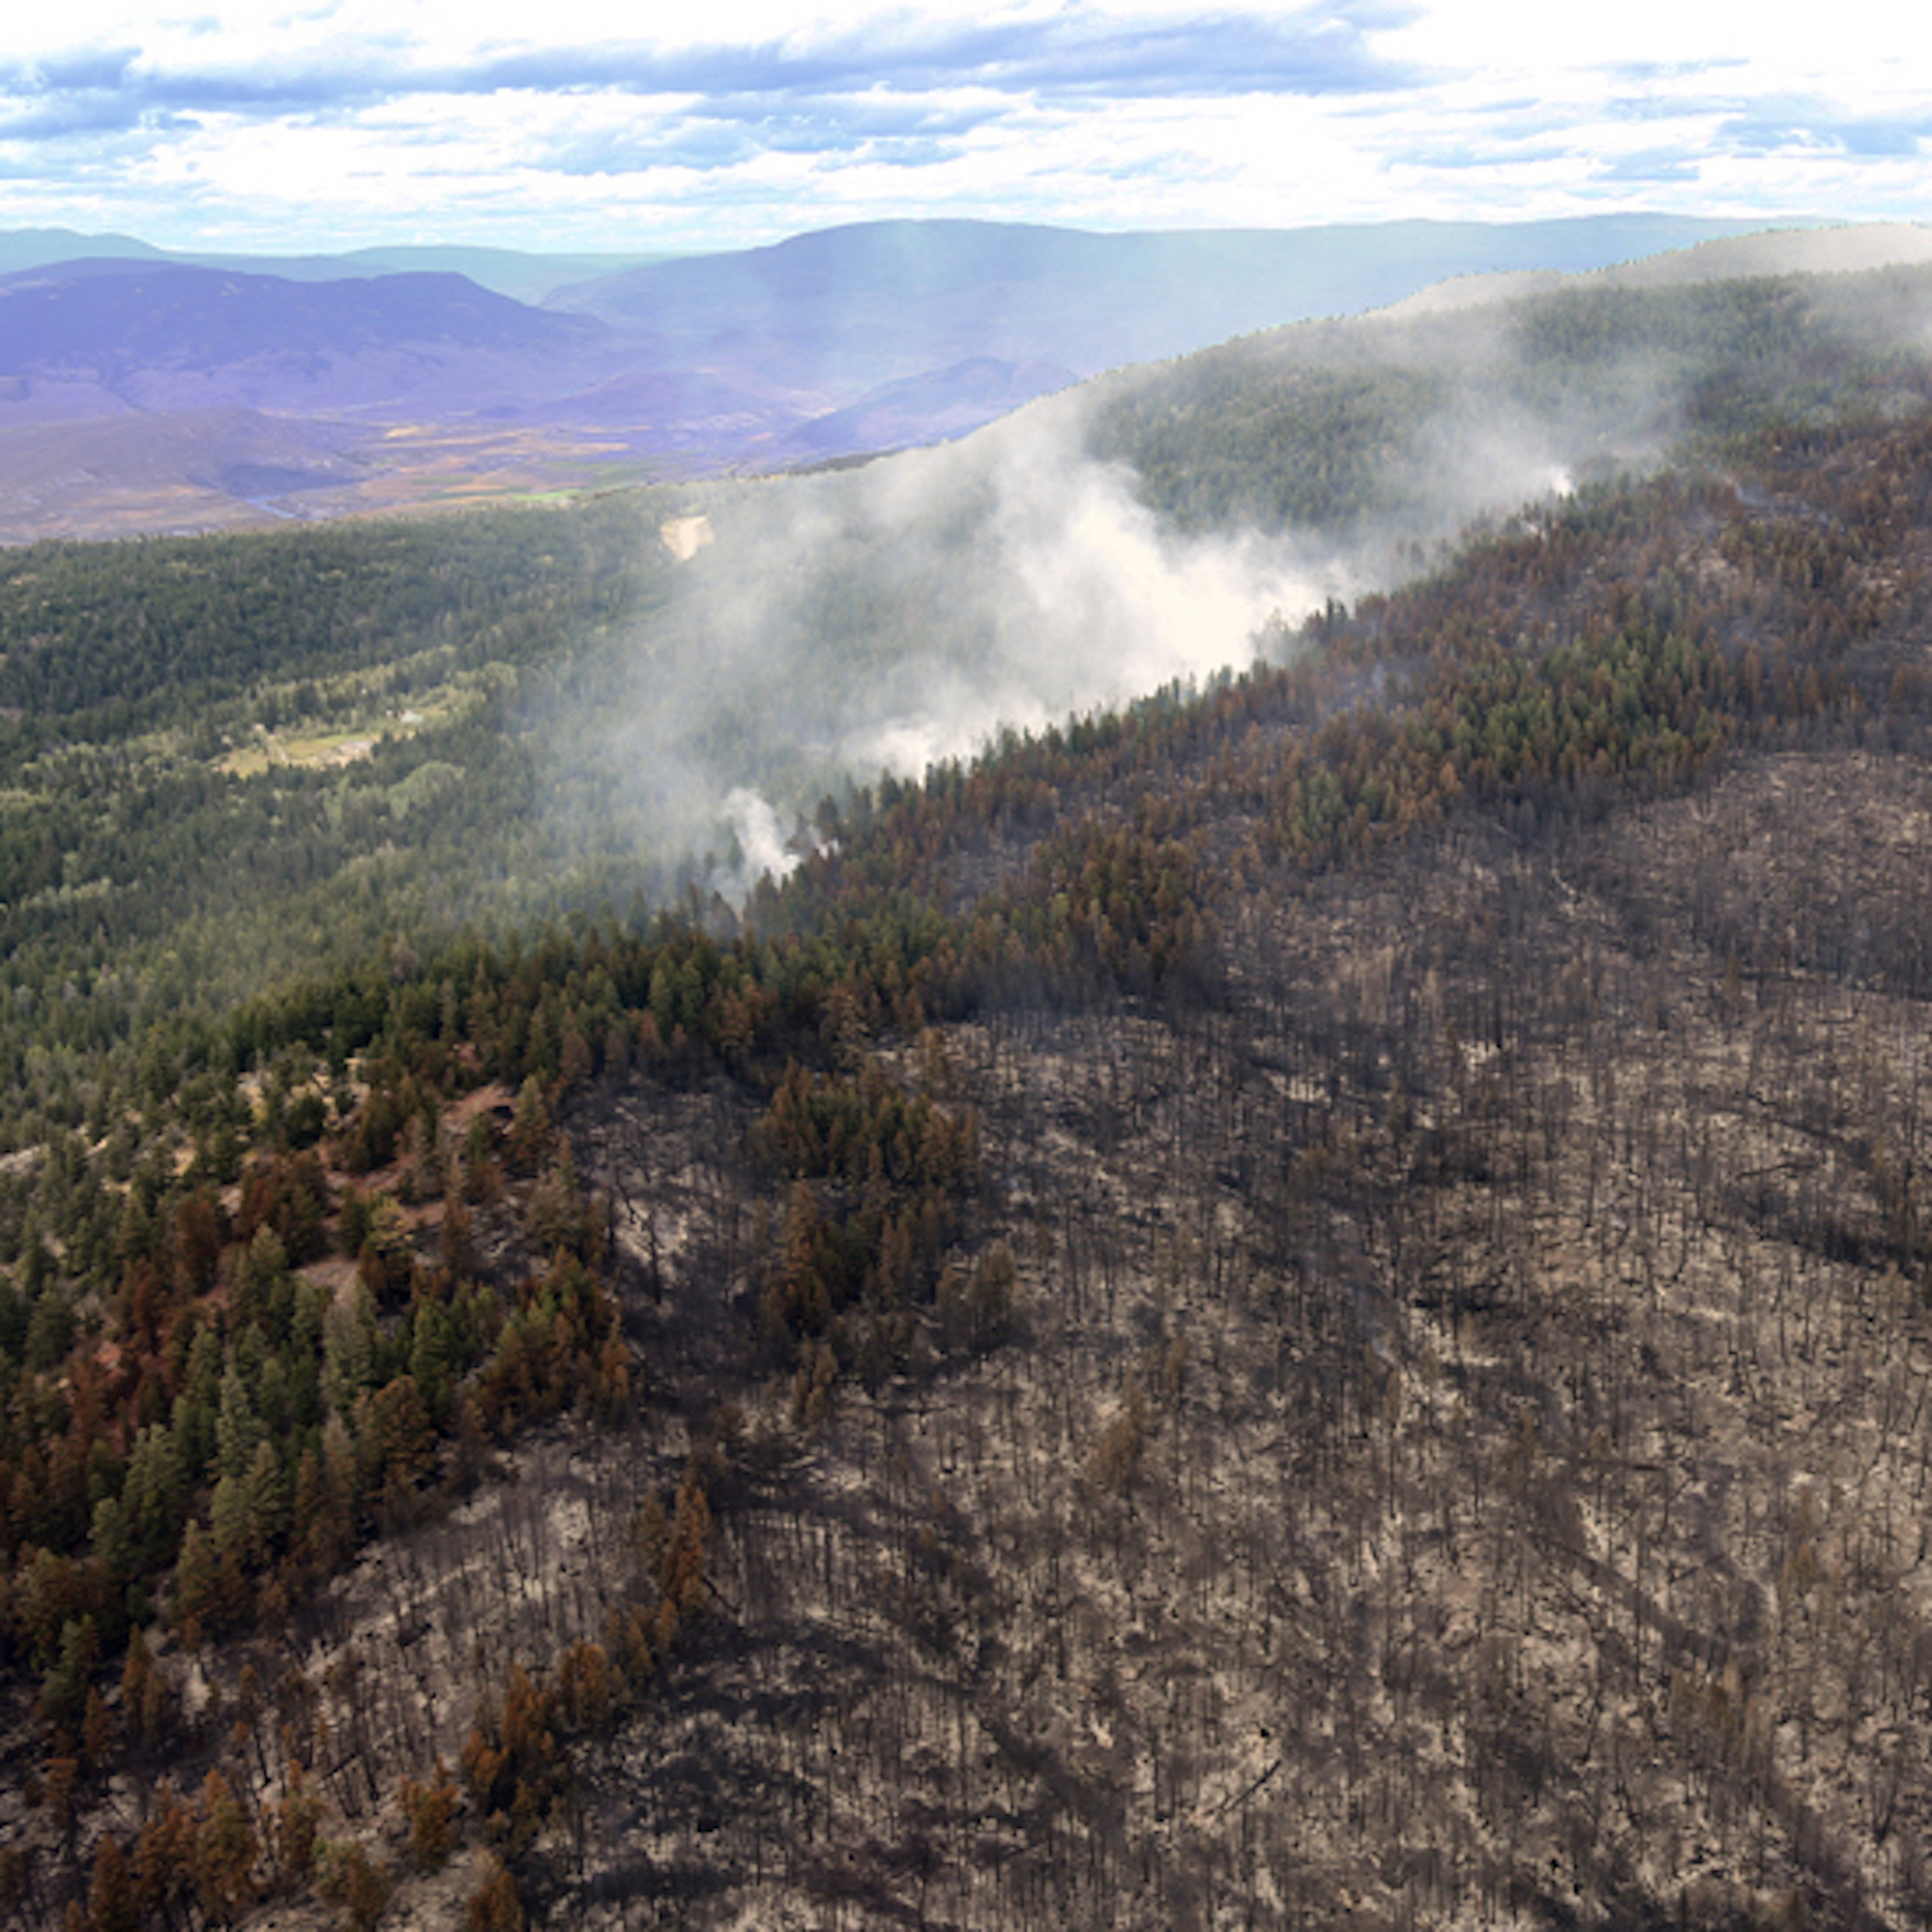
\includegraphics[scale=0.08]{figures/fire}\par
\end{columns}

\end{frame}

\begin{frame}{Aménagement forestier à différentes échelles spatiales}
\protect\hypertarget{amuxe9nagement-forestier-uxe0-diffuxe9rentes-uxe9chelles-spatiales}{}

Coupe sélective

\centering

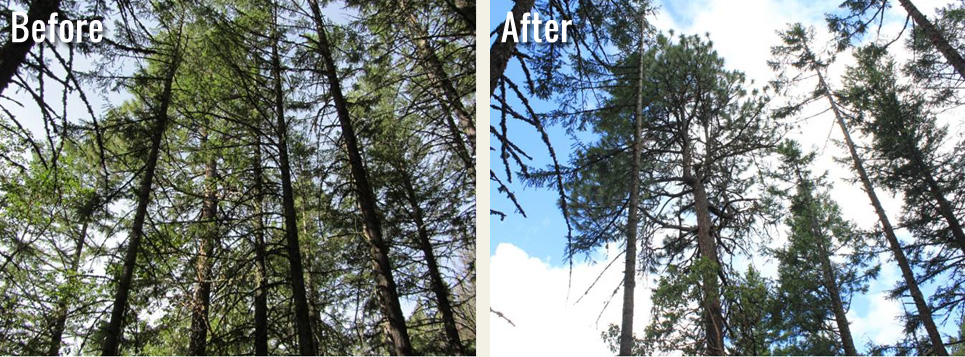
\includegraphics[scale=0.338]{figures/thinning}

\par

\end{frame}

\begin{frame}{Aménagement forestier à différentes échelles spatiales}
\protect\hypertarget{amuxe9nagement-forestier-uxe0-diffuxe9rentes-uxe9chelles-spatiales-1}{}

\vspace*{-7mm}

Plan de gestion

\centering

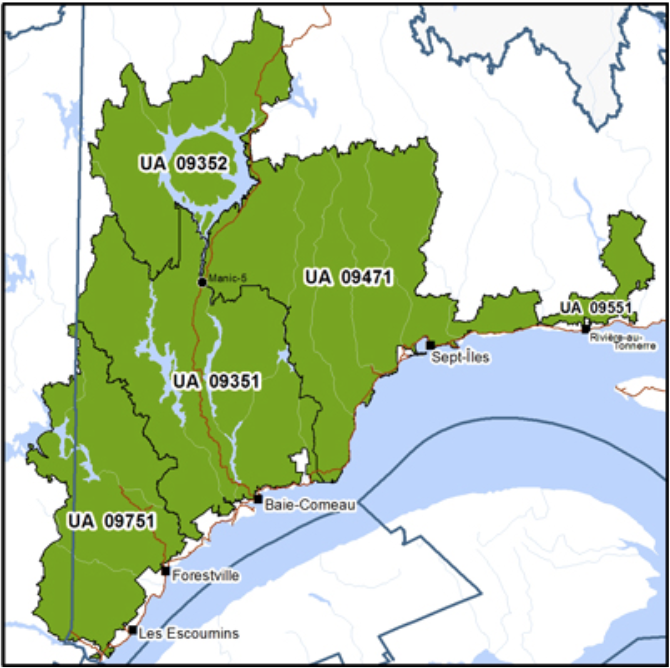
\includegraphics[scale=0.28]{figures/planGestion}

\par

\end{frame}

\begin{frame}{La démographie en tant que nœud central entre les
différentes échelles}
\protect\hypertarget{la-duxe9mographie-en-tant-que-nux153ud-central-entre-les-diffuxe9rentes-uxe9chelles}{}

\vspace*{-5mm}

Relier les taux vitaux aux dynamiques de population

\centering

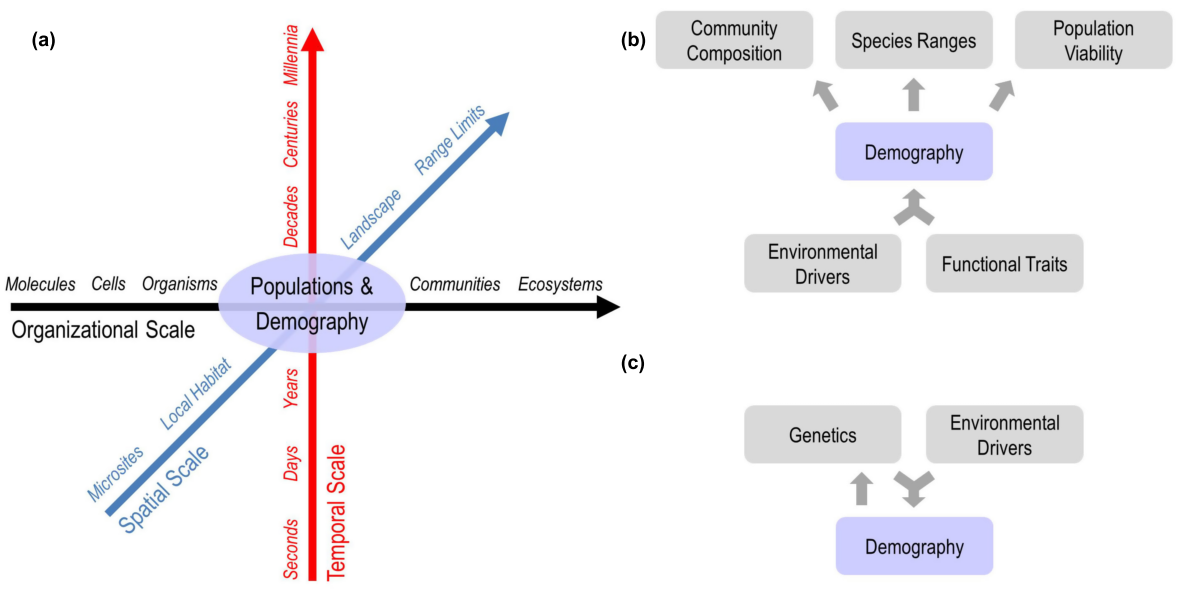
\includegraphics[scale=0.65]{figures/Griffith2016.png}

\par

\smallcitation{Griffith et al. 2016 J. Ecology}

\end{frame}

\begin{frame}{Objectifs}
\protect\hypertarget{objectifs-1}{}

\centering

Modèle de population structuré (IPM)

\begin{itemize}
\tightlist
\item
  Climat
\item
  Intéraction entre espèces
\item
  Modèle flexible
\item
  Questions theoriques et appliqués
\end{itemize}

\end{frame}

\begin{frame}{Modèle structuré à l’échelle locale}
\protect\hypertarget{moduxe8le-structuruxe9-uxe0-luxe9chelle-locale}{}

\begincols
\column{0.18\textwidth}
  \begin{itemize}
    \item
      {\color{plST}S}emence
    \item
      {\color{plST}J}uvénile
    \item
      {\color{plST}A}dulte
  \end{itemize}

\hfill\column{0.55\textwidth}
  \centering

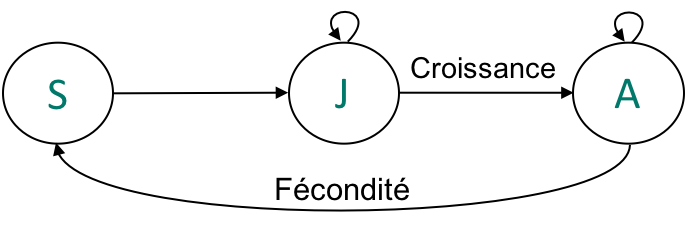
\includegraphics[scale=0.65]{figures/cycle}

\par
\stopcols

\end{frame}

\begin{frame}{Integral projection models (IPM)}
\protect\hypertarget{integral-projection-models-ipm}{}

\begincols
\column{0.5\textwidth}

\begin{align*}
    n(z', t + 1) = \int_{\Omega} \, \textbf{k(z', z)}\, n(z, t)\, \mathrm{d}x
  \end{align*}

\begin{align*}
    k(z', z) = \underbrace{[s(z)}_\text{Survie}\times\underbrace{g(z', z)]}_\text{Croissance} + \underbrace{F(z', z)}_\text{Fecundité}
  \end{align*}

\hfill\column{0.6\textwidth}
 \centering

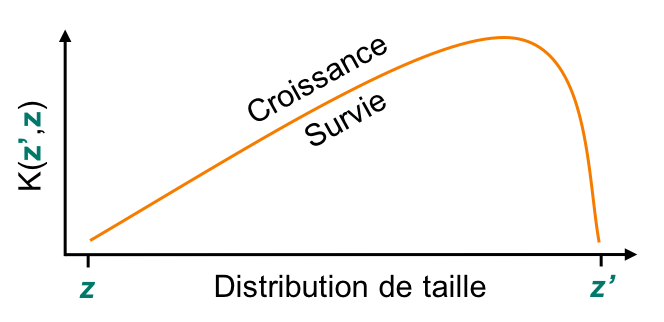
\includegraphics[scale=0.6]{figures/cycle_cont}

\par
\stopcols

\end{frame}

\begin{frame}{IPM - construction attendue}
\protect\hypertarget{ipm---construction-attendue}{}

\vspace*{-10mm}
\begin{center}
  \hspace*{-6mm}
  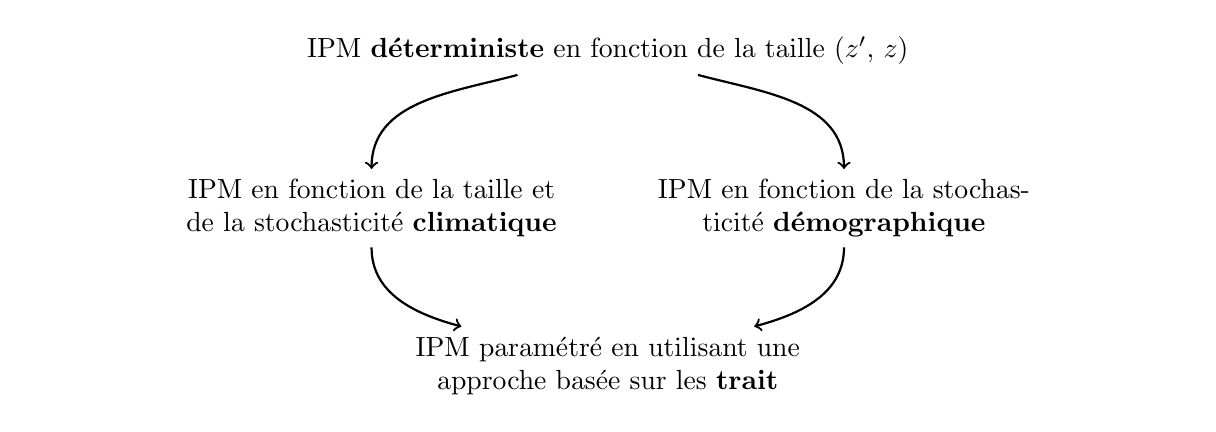
\begin{tikzpicture}[thick,every text node part/.style={align=center}]

    \node[text width=14.5cm] (n1) at (10,10.75) {IPM \textbf{déterministe} en fonction de la taille ($z'$, $z$)};

    \node[text width=5.5cm,visible on=<2->] (n2) at (7,8.75) {IPM en fonction de la taille et de la stochasticité \textbf{climatique} };
    \draw [->,visible on=<2->] (n1) edge [out=195, in=90] (n2);

    \node[text width=5cm,visible on=<3->] (n3) at (13,8.75) {IPM en fonction de la stochasticité \textbf{démographique}};
    \draw [->,visible on=<3->] (n1) edge [out=345, in=90] (n3);

    \node[text width=7cm,visible on=<4->] (n4) at (10,6.75) {IPM paramétré en utilisant une approche basée sur les \textbf{trait}};
    \draw [->,visible on=<4->] (n2) edge [out=270, in=165] (n4);
    \draw [->,visible on=<4->] (n3) edge [out=270, in=15] (n4);

  \end{tikzpicture}
\end{center}


\end{frame}

\hypertarget{chapitre-iii-effet-du-climat-et-des-interactions-biotiques-sur-la-dynamique-daire-de-ruxe9partition-des-espuxe8ces}{%
\section{\texorpdfstring{Chapitre III: \newline Effet du climat et des
interactions biotiques sur la dynamique d’aire de répartition des
espèces}{Chapitre III: Effet du climat et des interactions biotiques sur la dynamique d’aire de répartition des espèces}}\label{chapitre-iii-effet-du-climat-et-des-interactions-biotiques-sur-la-dynamique-daire-de-ruxe9partition-des-espuxe8ces}}

\begin{frame}{Dynamique au niveau de la population}
\protect\hypertarget{dynamique-au-niveau-de-la-population}{}

Des taux vitaux determinent l’air de répartition des espèces

\centering

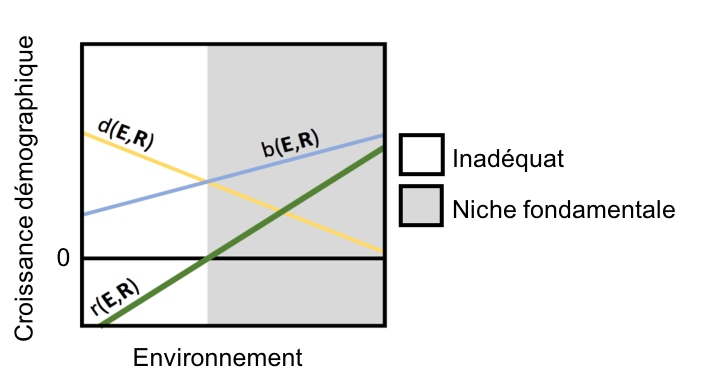
\includegraphics[scale=0.685]{figures/Godsoe2017a.png}

\par

\smallcitation{Godsoe et al. 2017 Trends Ecol. Evol.}

\end{frame}

\begin{frame}{Dynamique au niveau de la communauté}
\protect\hypertarget{dynamique-au-niveau-de-la-communautuxe9}{}

Et l’interaction entre espéces determine-t-elle aussi l’air de
répartition des espèces ?

\centering

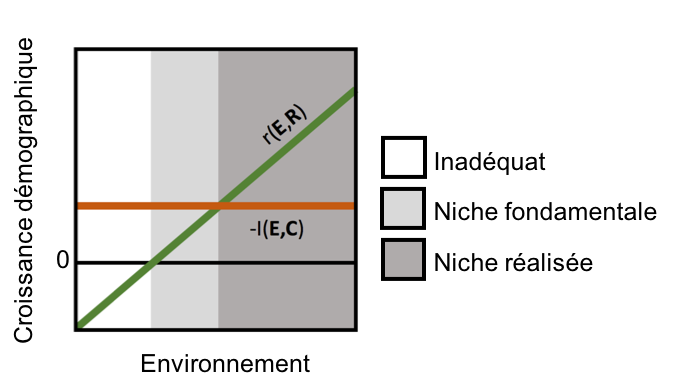
\includegraphics[scale=0.685]{figures/Godsoe2017b.png}

\par

\smallcitation{Godsoe et al. 2017 Trends Ecol. Evo.}

\end{frame}

\begin{frame}{Objectifs}
\protect\hypertarget{objectifs-2}{}

\centering

Tester l’effet du \textbf{climat} et de l’\textbf{interaction entre
spèces} sur le taux de croissance, et comment ces effets locaux évoluent
à l’échelle régionale ?

\begin{enumerate}
[1.]
\tightlist
\item
  Taux vitaux

  \begin{itemize}
  \tightlist
  \item
    Interaction entre espèces
  \item
    Climat
  \end{itemize}
\end{enumerate}

\end{frame}

\begin{frame}{Objectifs - Résultats attendus}
\protect\hypertarget{objectifs---ruxe9sultats-attendus}{}

\centering

Comment le taux de croissance et la force d’intraction entre espèces
varient sur un gradient environnementale ?

\vspace*{10mm}

\centering 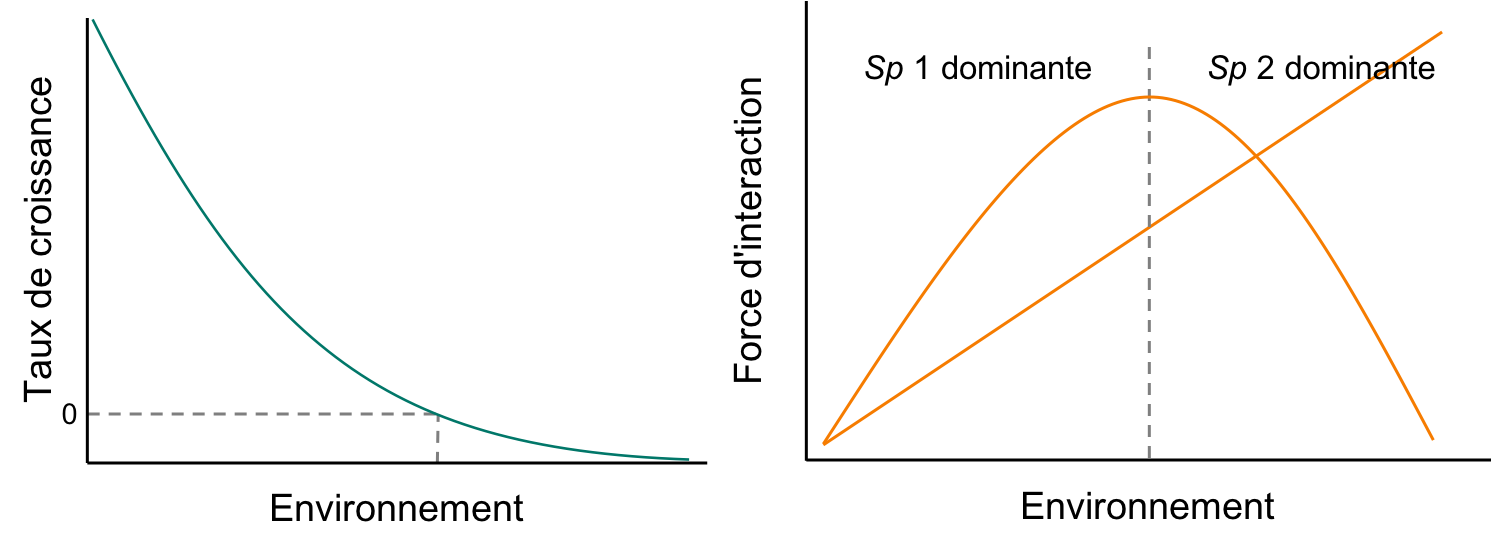
\includegraphics[scale=0.45]{figures/output_chap2a.png}

\par

\end{frame}

\begin{frame}{Objectifs - Résultats attendus}
\protect\hypertarget{objectifs---ruxe9sultats-attendus-1}{}

\centering

\emph{Quelle est la part relative des interactions biotiques et du le
climat dans la définition de la limite de l’aire de répartition ?}

\vspace*{10mm}
\centering

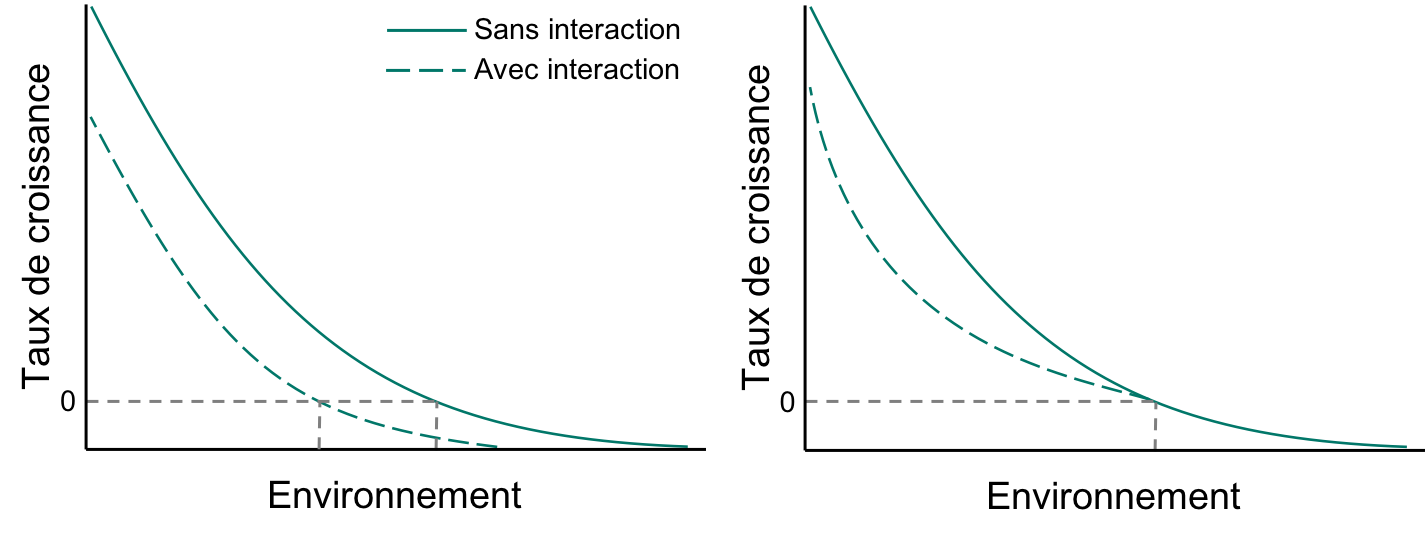
\includegraphics[scale=0.45]{figures/output_chap2b.png}

\par

\end{frame}

\hypertarget{chapitre-iv-effet-de-lamuxe9nagement-forestier-sur-le-taux-de-croissance-des-espuxe8ces-consuxe9quences-pour-la-productivituxe9}{%
\section{\texorpdfstring{Chapitre IV: \newline Effet de l’aménagement
forestier sur le taux de croissance des espèces
\newline \large Conséquences pour la
productivité}{Chapitre IV: Effet de l’aménagement forestier sur le taux de croissance des espèces Conséquences pour la productivité}}\label{chapitre-iv-effet-de-lamuxe9nagement-forestier-sur-le-taux-de-croissance-des-espuxe8ces-consuxe9quences-pour-la-productivituxe9}}

\begin{frame}{Effets de l’aménagement forestier}
\protect\hypertarget{effets-de-lamuxe9nagement-forestier}{}

\begincols
\centering
\column{0.5\textwidth}
  \centering

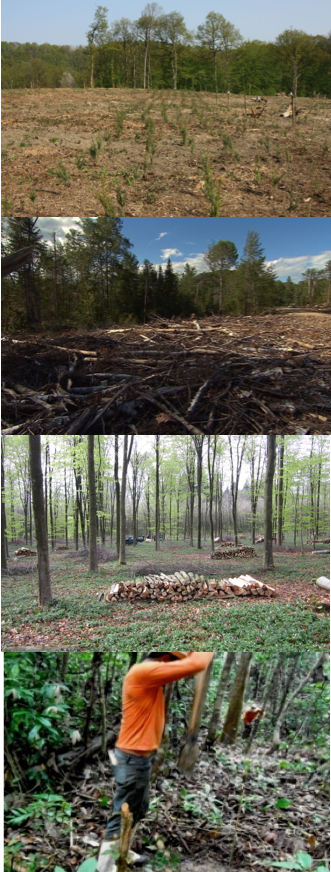
\includegraphics[scale=0.50]{figures/managPrac}

\par
\hfill\column{0.2\textwidth}
  \begin{itemize}
    \item
      \vspace*{-8mm}
      Colonisation
    \item
      \vspace*{11mm}
      Pertubation
    \item
      \vspace*{11mm}
      Coexistence
    \item
      \vspace*{11mm}
      Competition
  \end{itemize}
\hfill\column{0.4\textwidth}
  \vspace*{-15mm}

\begin{gather*}
  \text{Croissance} \times \text{Survie} = \alert{r}
  \end{gather*} \stopcols

\end{frame}

\begin{frame}{Effets de l’aménagement forestier - Coupe sélective}
\protect\hypertarget{effets-de-lamuxe9nagement-forestier---coupe-suxe9lective}{}

\begincols
\hspace*{20mm}
\column{0.5\textwidth}

\textbf{Positif}

\begin{itemize}
    \item
      Disponibilité de la lumière
    \item
      Disponibilité en eau du soil
    \item
      Azote
  \end{itemize}
\hfill\column{0.5\textwidth}
  \vspace*{-10mm}

\textbf{Negatif}

\begin{itemize}
    \item
      Habitat disponible
    \item
      Invasion d'ericacées
  \end{itemize}
\stopcols

\end{frame}

\begin{frame}{Objectifs}
\protect\hypertarget{objectifs-3}{}

\centering

Tester l’impact de l’\textbf{aménagement forestier} sur le \textbf{taux
de croissance} des arbres et la rélation entre le taux de croissance et
la \textbf{productivité} forestier

\begin{enumerate}
[1.]
\tightlist
\item
  Taux vitaux

  \begin{itemize}
  \tightlist
  \item
    Interaction entre espèces
  \item
    Climat
  \end{itemize}
\end{enumerate}

\end{frame}

\begin{frame}{Objectifs - Résultats attendus}
\protect\hypertarget{objectifs---ruxe9sultats-attendus-2}{}

\centering

\emph{Comment les pratiques d’aménagement interagissent avec les taux
vitaux de la population dans un contexte de changement climatique et
d’interaction entre les espèces ?}

\vspace*{10mm}
\centering

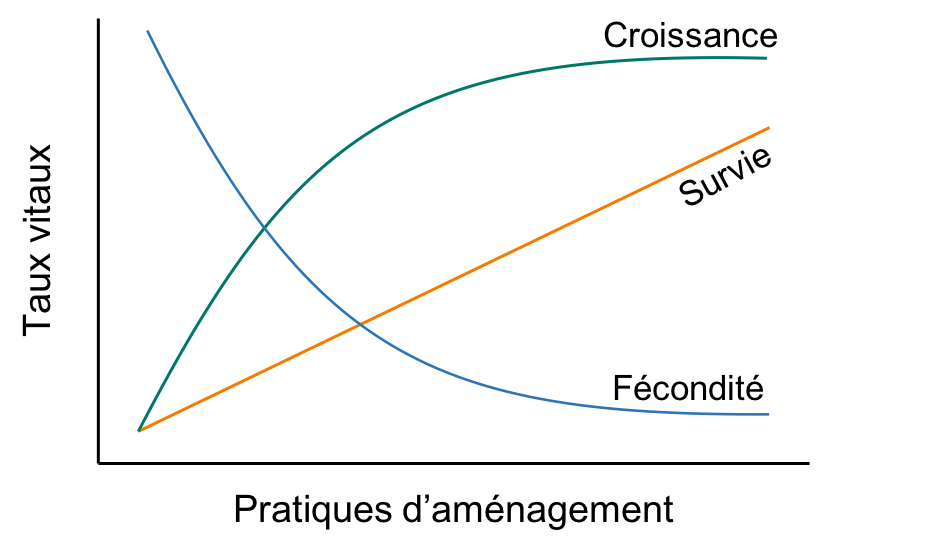
\includegraphics[scale=0.45]{figures/output_chap3a.png}

\par

\end{frame}

\begin{frame}{Objectifs - Résultats attendus}
\protect\hypertarget{objectifs---ruxe9sultats-attendus-3}{}

\centering

\emph{Quelles sont les régions cibles pour l’aménagement forestier ?}

\centering

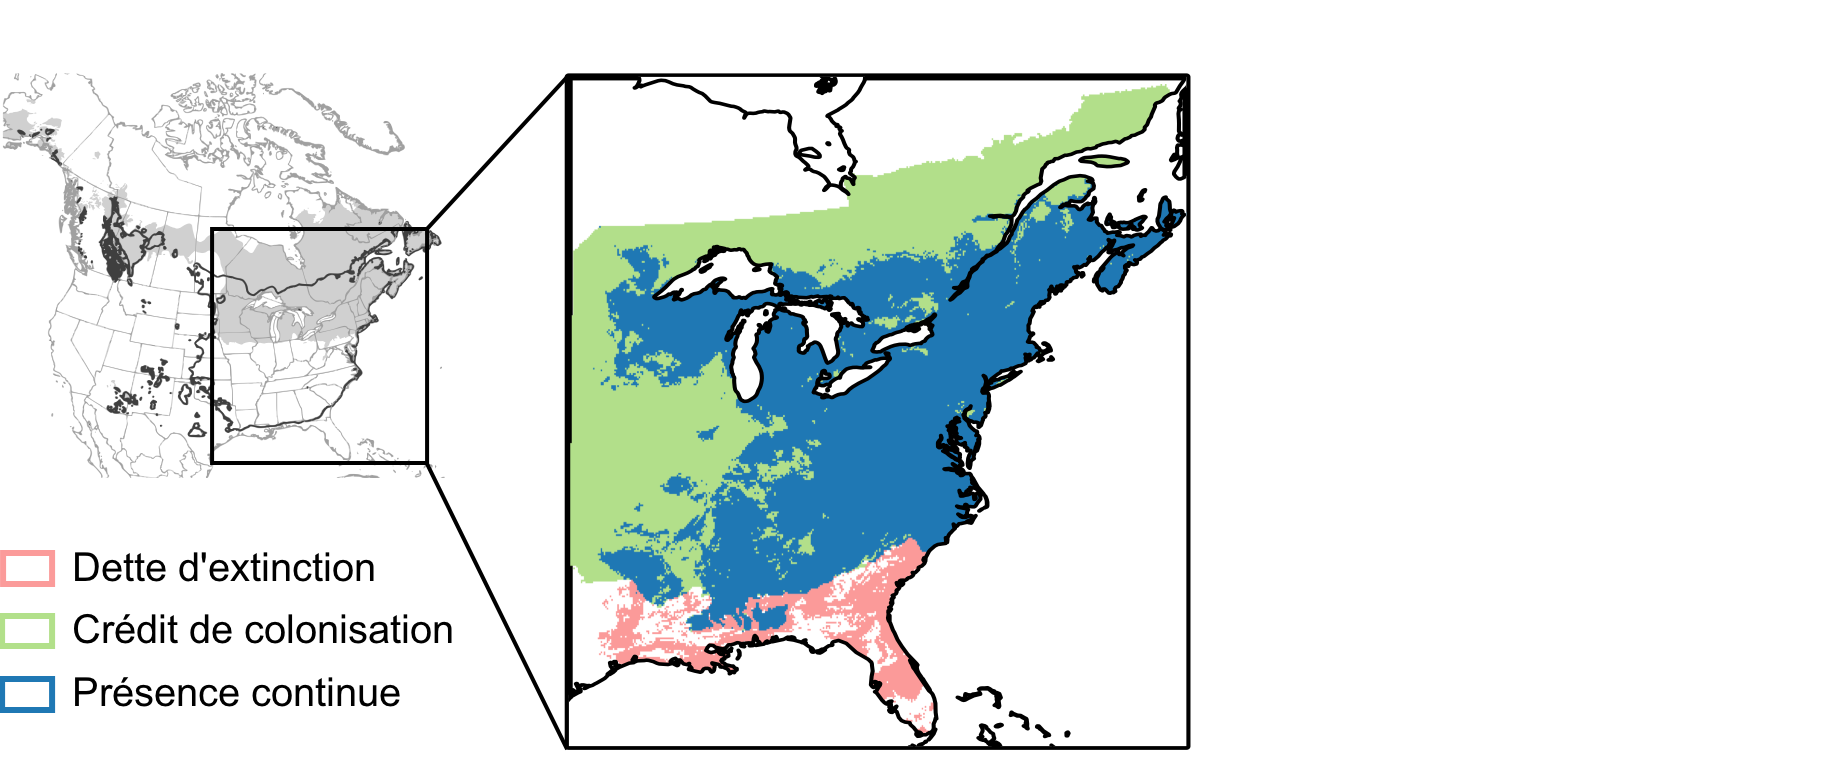
\includegraphics[scale=0.4]{figures/Talluto0.png}\hspace*{-4cm}

\par

\end{frame}

\hypertarget{conclusion}{%
\section{Conclusion}\label{conclusion}}

\begin{frame}{Contributions possibles du projet}
\protect\hypertarget{contributions-possibles-du-projet}{}

\begin{enumerate}
[1.]
\item
  Potential de l’aménagement forestier à une échelle réginale
\item
  \textbf{IPM}: approche par trait

  \begin{itemize}
  \tightlist
  \item
    Vers une approche plus modulaire
  \end{itemize}
\item
  Interaction \textbf{taux de croissance} locale X \textbf{dynamique
  d’air de répartition} régionale

  \begin{itemize}
  \tightlist
  \item
    Vers une approche integrative
  \end{itemize}
\item
  Effet de l’\textbf{aménagement forestier} sur le \textbf{taux de
  croissance}
\end{enumerate}

\end{frame}

\begin{frame}[plain]{}
\protect\hypertarget{section}{}

\plain{Obrigado!}

\end{frame}

\begin{frame}[plain]
  \begin{picture}(0,0)
    \put(-28.5,-175){%
      \pgfuseimage{titlebackground}
    }
  \end{picture}
\end{frame}

\end{document}
